\documentclass[10pt]{beamer}

\usetheme[progressbar=frametitle]{metropolis}
\usepackage{appendixnumberbeamer}

\makeatletter
\definecolor{uosblue}{RGB}{10, 77, 155}
\setbeamercolor{background canvas}{bg=white}
%\setbeamercolor{normal text}{fg=lightbeige}
\setbeamercolor{frametitle}{bg=uosblue}
\setbeamercolor{progress bar}{fg=black, bg=lightgray}
\setbeamercolor{section in head}{bg=white}
\setlength{\metropolis@titleseparator@linewidth}{2pt}
\setlength{\metropolis@progressonsectionpage@linewidth}{2pt}
\setlength{\metropolis@progressinheadfoot@linewidth}{2pt}
\makeatother

%\definecolor{links}{HTML}{00FFFF}
\hypersetup{colorlinks,linkcolor=,urlcolor=uosblue}


%\usepackage{appendixnumberbeamer}

\usepackage{booktabs}
\usepackage[scale=2]{ccicons}
\usepackage{pgfplots}
\usepgfplotslibrary{dateplot}
\usepackage{xspace}
%\usepackage[utf8]{inputenc}
\usepackage{feynmf}
\usepackage{amsmath}
%\usepackage{subfig}
\usepackage{caption}
\usepackage{subcaption}
\usepackage{comment}

%\usepackage{enumitem} % itemize indentation



% https://pt.overleaf.com/learn/latex/Code_Highlighting_with_minted
\usepackage{minted}
\setminted[python]{ %
    linenos=false,
    autogobble=true,          % Automatically remove common white space
    frame=lines,
    framesep=2mm,
    % fontsize=\footnotesize
}

\usepackage{physics}

\newcommand{\textGeV}[0]{\text{GeV}}
\newcommand{\textjet}[0]{\text{jet}}
\newcommand{\saja}[0]{\textsc{SaJa}}

\definecolor{JetGreen}{RGB}{2, 115, 94}
\definecolor{PartonViolet}{RGB}{117, 89, 217}

%%%%%%%%%%%%%%%%%%%%%%%%%%%%%%%%%%%%%%%%%%%%%%%%%%%%%%%%%%%%%%%%%%

\title{Zero-Permutation Jet-Parton Assignment}

\subtitle{Top quark pair reconstruction using an attention-based neural network}

\author{
    Jason Sang Hun Lee,
    Inkyu Park,
    Ian James Watson,
    and \underline{Seungjin Yang} \\
    University of Seoul % positioning problem
}

%\institute[VFU]{University of Seoul}

\date{
    4th Inter-experiment Machine Learning Workshop\\
    October 21, 2020
}

\titlegraphic{\hfill
\includegraphics[height=1.5cm]{figures/misc/logo.png}}

%\logo{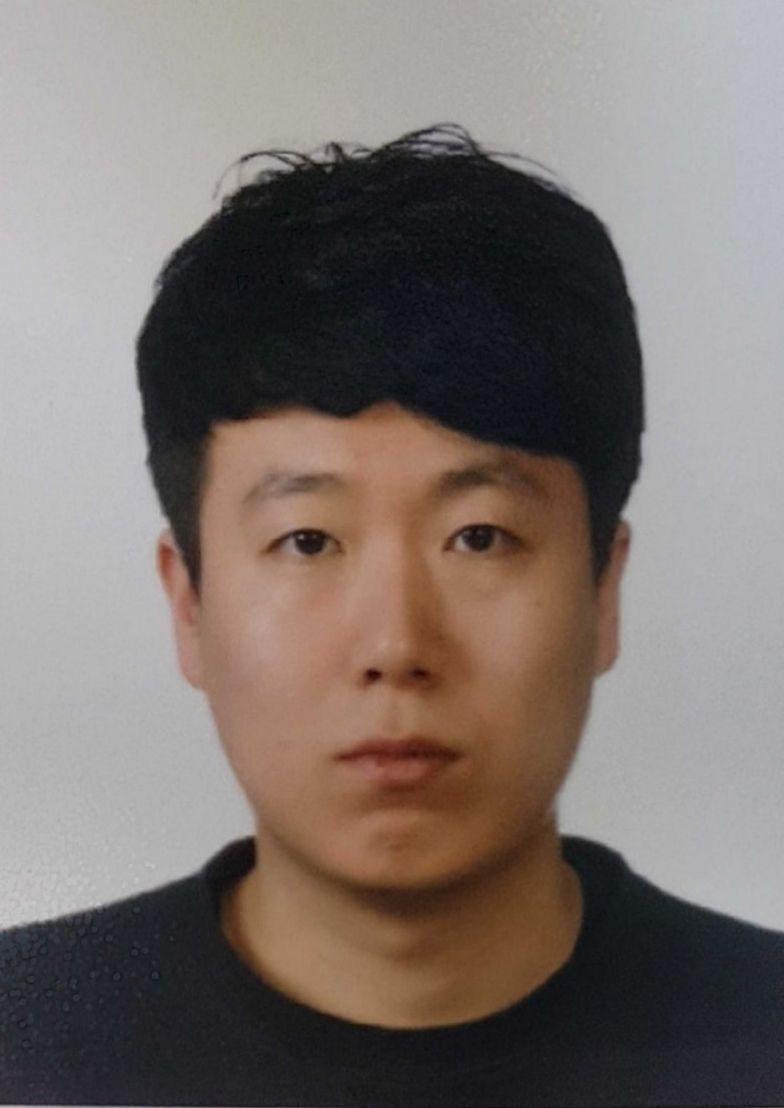
\includegraphics[height=2cm]{figures/misc/photo_2020-07-03_19-28-55.jpg}}

\begin{document}

%\begin{frame}{}
\maketitle
%\end{frame}




%%%%%%%%%%%%%%%%%%%%%%%%%%%%%%%%%%%%%%%%%%%%%%%%%%%%%%%%%%%%%%%%%%%%%%%%%%%%%%%%
\begin{frame}[fragile]{Introduction}
\begin{columns}
    \column{0.65\textwidth}
    \begin{itemize}
        \item[$\bullet$] The reconstruction of events with intermediate states decaying to jets requires a technique to assign jets to partons.
        \item[$\bullet$] The number of jets can be greater than the number of partons because of additional QCD radiation. It makes the assignment harder.
        \item[$\bullet$] We introduce \textbf{the self-attention for jet assignment (\saja ) network without requiring jet permutations}. We apply \saja\, to find jet-parton assignments of fully-hadronic $t\bar{t}$ events to test the performance.
    \end{itemize}

    \column{0.35\textwidth}
    % https://wiki.physik.uzh.ch/cms/latex:feynman#top_quark_pair_decay_into_a_w_boson_pair_and_a_b_quark_pair
    \begin{fmffile}{feyngraph}
    \begin{fmfgraph*}(100,100)
        \fmfset{arrow_len}{3.5mm}
        \fmfstraight
        \fmfleft{i1,i2,i3,i4,i5}
        \fmfright{o1,o2,o3,o4,o5,o6}
        % qq -> g
        \fmf{fermion,tension=1.5}{i4,vg,i2}
        \fmf{gluon,tension=1.5}{vtt,vg}
        \fmf{phantom,tension=0.5}{o3,vtt,o4} % balance
        \fmflabel{$\bar{q}$}{i2}
        \fmflabel{$q$}{i4}
        \fmffreeze
        % tt
        \fmf{fermion,tension=1.2}{v1,vtt,v2}  % top quark pair
        \fmf{phantom,label={$\bar{\text{t}}$},tension=0,label.side=right}{vtt,v1} % top label
        \fmf{phantom,label={$\text{t}$},tension=0,label.side=left}{vtt,v2} % top label
        \fmf{phantom,tension=1}{o1,v1,o2} % balance
        \fmf{phantom,tension=1}{o5,v2,o6} % balance
        \fmf{phantom,tension=0.5}{i1,v1,v2,i5} % balance
        \fmffreeze
        % bW -> bqq
        \fmf{boson,tension=0.8,label={$\text{W}^+$},label.side=right}{v2,v21}  % W boson
        \fmf{fermion,tension=1.2,fore=red}{v2,o6} % b quark
        \fmf{fermion}{o5,v21,o4}
        % bW -> blnu
        \fmf{boson,tension=1.4,label={$\text{W}^-$},label.side=right}{v1,v11}  % W boson
        \fmf{fermion,tension=0.5}{v1,o3} % b quark
        \fmf{fermion}{o1,v11,o2}
        \fmflabel{\makebox[3.2mm][l]{q}}{o1}
        \fmflabel{\makebox[3.2mm][l]{$\bar{\text{q}}'$}}{o2}
        \fmflabel{$\bar{\text{b}}$}{o3}
        \fmflabel{\makebox[3.2mm][l]{$\bar{\text{q}}'$}}{o4}
        \fmflabel{\makebox[3.2mm][l]{q}}{o5}
        \fmflabel{$\text{b}$}{o6}
    \end{fmfgraph*}
    \end{fmffile}
\end{columns}
\end{frame}

%%%%%%%%%%%%%%%%%%%%%%%%%%%%%%%%%%%%%%%%%%%%%%%%%%%%%%%%%%%%%%%%%%%%%%%%%%%%%%%%
\begin{frame}[fragile]{Preceding Research}
    \begin{block}{$\blacksquare$ $\chi^{2}$ method {\scriptsize \href{https://link.springer.com/article/10.1140\%2Fepjc\%2Fs10052-019-6788-2}{[CMS, Eur. Phys. J. C 79 (2019) 313]}}}
        \centering
        \smallskip
        \scalebox{.85}{$
            \chi^{2}=\sum_{j\in\text{jets}} [
                \frac{ ( p_{T,j}^{ \text{reco} } - p_{T,j}^{ \text{fit} } )^{2} }{ \sigma_{p_{T,j}^{2}} }
                - \frac{ ( \eta_{j}^{ \text{reco} } - \eta_{j}^{ \text{fit} } )^{2} }{ \sigma_{\eta_{j}^{2}} }
                - \frac{ ( \phi_{j}^{ \text{reco} } - \phi_{j}^{ \text{fit} } )^{2} }{ \sigma_{\eta_{j}^{2}} }
            ]
        $}
    \end{block}
    
    \begin{block}{$\blacksquare$ Kinematic likelihood fitting {\scriptsize \href{https://www.sciencedirect.com/science/article/pii/S0168900214001855?via\%3Dihub}{[J. Erdmann, Nucl.Instrum.Meth.A 748 (2014) 18-25]}}}
        \centering
        \smallskip
        \scalebox{.7}{$
            \mathcal{L} = B(m_{q_{1}q_{2}q_{3}}|m_{t},\Gamma_{t}) \cdot
                         B(m_{q_{1}q_{2}}|m_{W},\Gamma_{W}) \cdot
                         B(m_{q_{4}q_{5}q_{6}}|m_{t},\Gamma_{t}) \cdot
                         B(m_{q_{4}q_{5}}|m_{W},\Gamma_{W}) \cdot
                         \prod_{i=1}^{6} W_{\text{jet}}(E_{\text{jet},i}^{\text{meas}}|E_{\text{jet},i})
        $}
    \end{block}

    \begin{block}{$\blacksquare$ Machine Learning {\tiny \href{https://iopscience.iop.org/article/10.1088/1748-0221/12/08/P08020}{[M. Erdmann, JINST 12 (2017) P08020]}, \href{https://iopscience.iop.org/article/10.1088/1748-0221/14/11/P11015}{[J. Erdmann, JINST 14 (2019) P11015]}}}
        $${\footnotesize \text{correct or wrong} = \text{model}(\text{assignment})}$$
    \end{block}
    
    %\noindent{\color{uosblue} \rule{\linewidth}{0.5mm} }
    
    All of the above methods follow the same steps.
    \begin{itemize}
        \item[1] Compute all (promising) jet permutations.
        \item[2] Evaluate how well each permutation agrees with the underlying event topology.  {(\scriptsize $\chi^{2}, \mathcal{L},$ the sigmoid output of NN, BDT score)}
        \item[3] Choose the best permutation.
    \end{itemize}
    
    $\Rightarrow$ Combinatorial explosion O(n!)
\end{frame}


%%%%%%%%%%%%%%%%%%%%%%%%%%%%%%%%%%%%%%%%%%%%%%%%%%%%%%%%%%%%%%%%%%%%%%%%%%%%%%%%
\begin{frame}[fragile]{Modeling}
    Jet-parton assignment as jet-wise classification.\break
    \begin{equation*}
        \small
        f^{\theta}: 
        \begin{bmatrix}
            \mathbf{x}^{(1)} \\
            \vdots \\
            \mathbf{x}^{(N)}
        \end{bmatrix}
        \rightarrow
        \begin{bmatrix}
            \hat{y}^{(1)}_{b_{1}} & \hat{y}^{(1)}_{W_{1}} & \hat{y}^{(1)}_{b_{2}} & \hat{y}^{(1)}_{W_{2}} & \hat{y}^{(1)}_{\textrm{other}} \\
            \vdots & \vdots & \vdots & \vdots & \vdots \\
            \hat{y}^{(N)}_{b_{1}} & \hat{y}^{(N)}_{W_{1}} & \hat{y}^{(N)}_{b_{2}} & \hat{y}^{(N)}_{W_{2}} & \hat{y}^{(N)}_{\textrm{other}}
        \end{bmatrix}
    \end{equation*}
 
    \begin{itemize}
        \item {\footnotesize Since it is hard to distinguish jets originating from $t$ and jets originating from $\bar{t}$, arbitrary indices 1 and 2 are introduced.}
        \item {\footnotesize When the assignment doesn't agree with the underlying topology (e.g. no $b_{1}$ or 3 $ W_{2}$), the assignment is said to be topologically invalid and is not selected.}
    \end{itemize}

    \begin{figure}
        \centering
        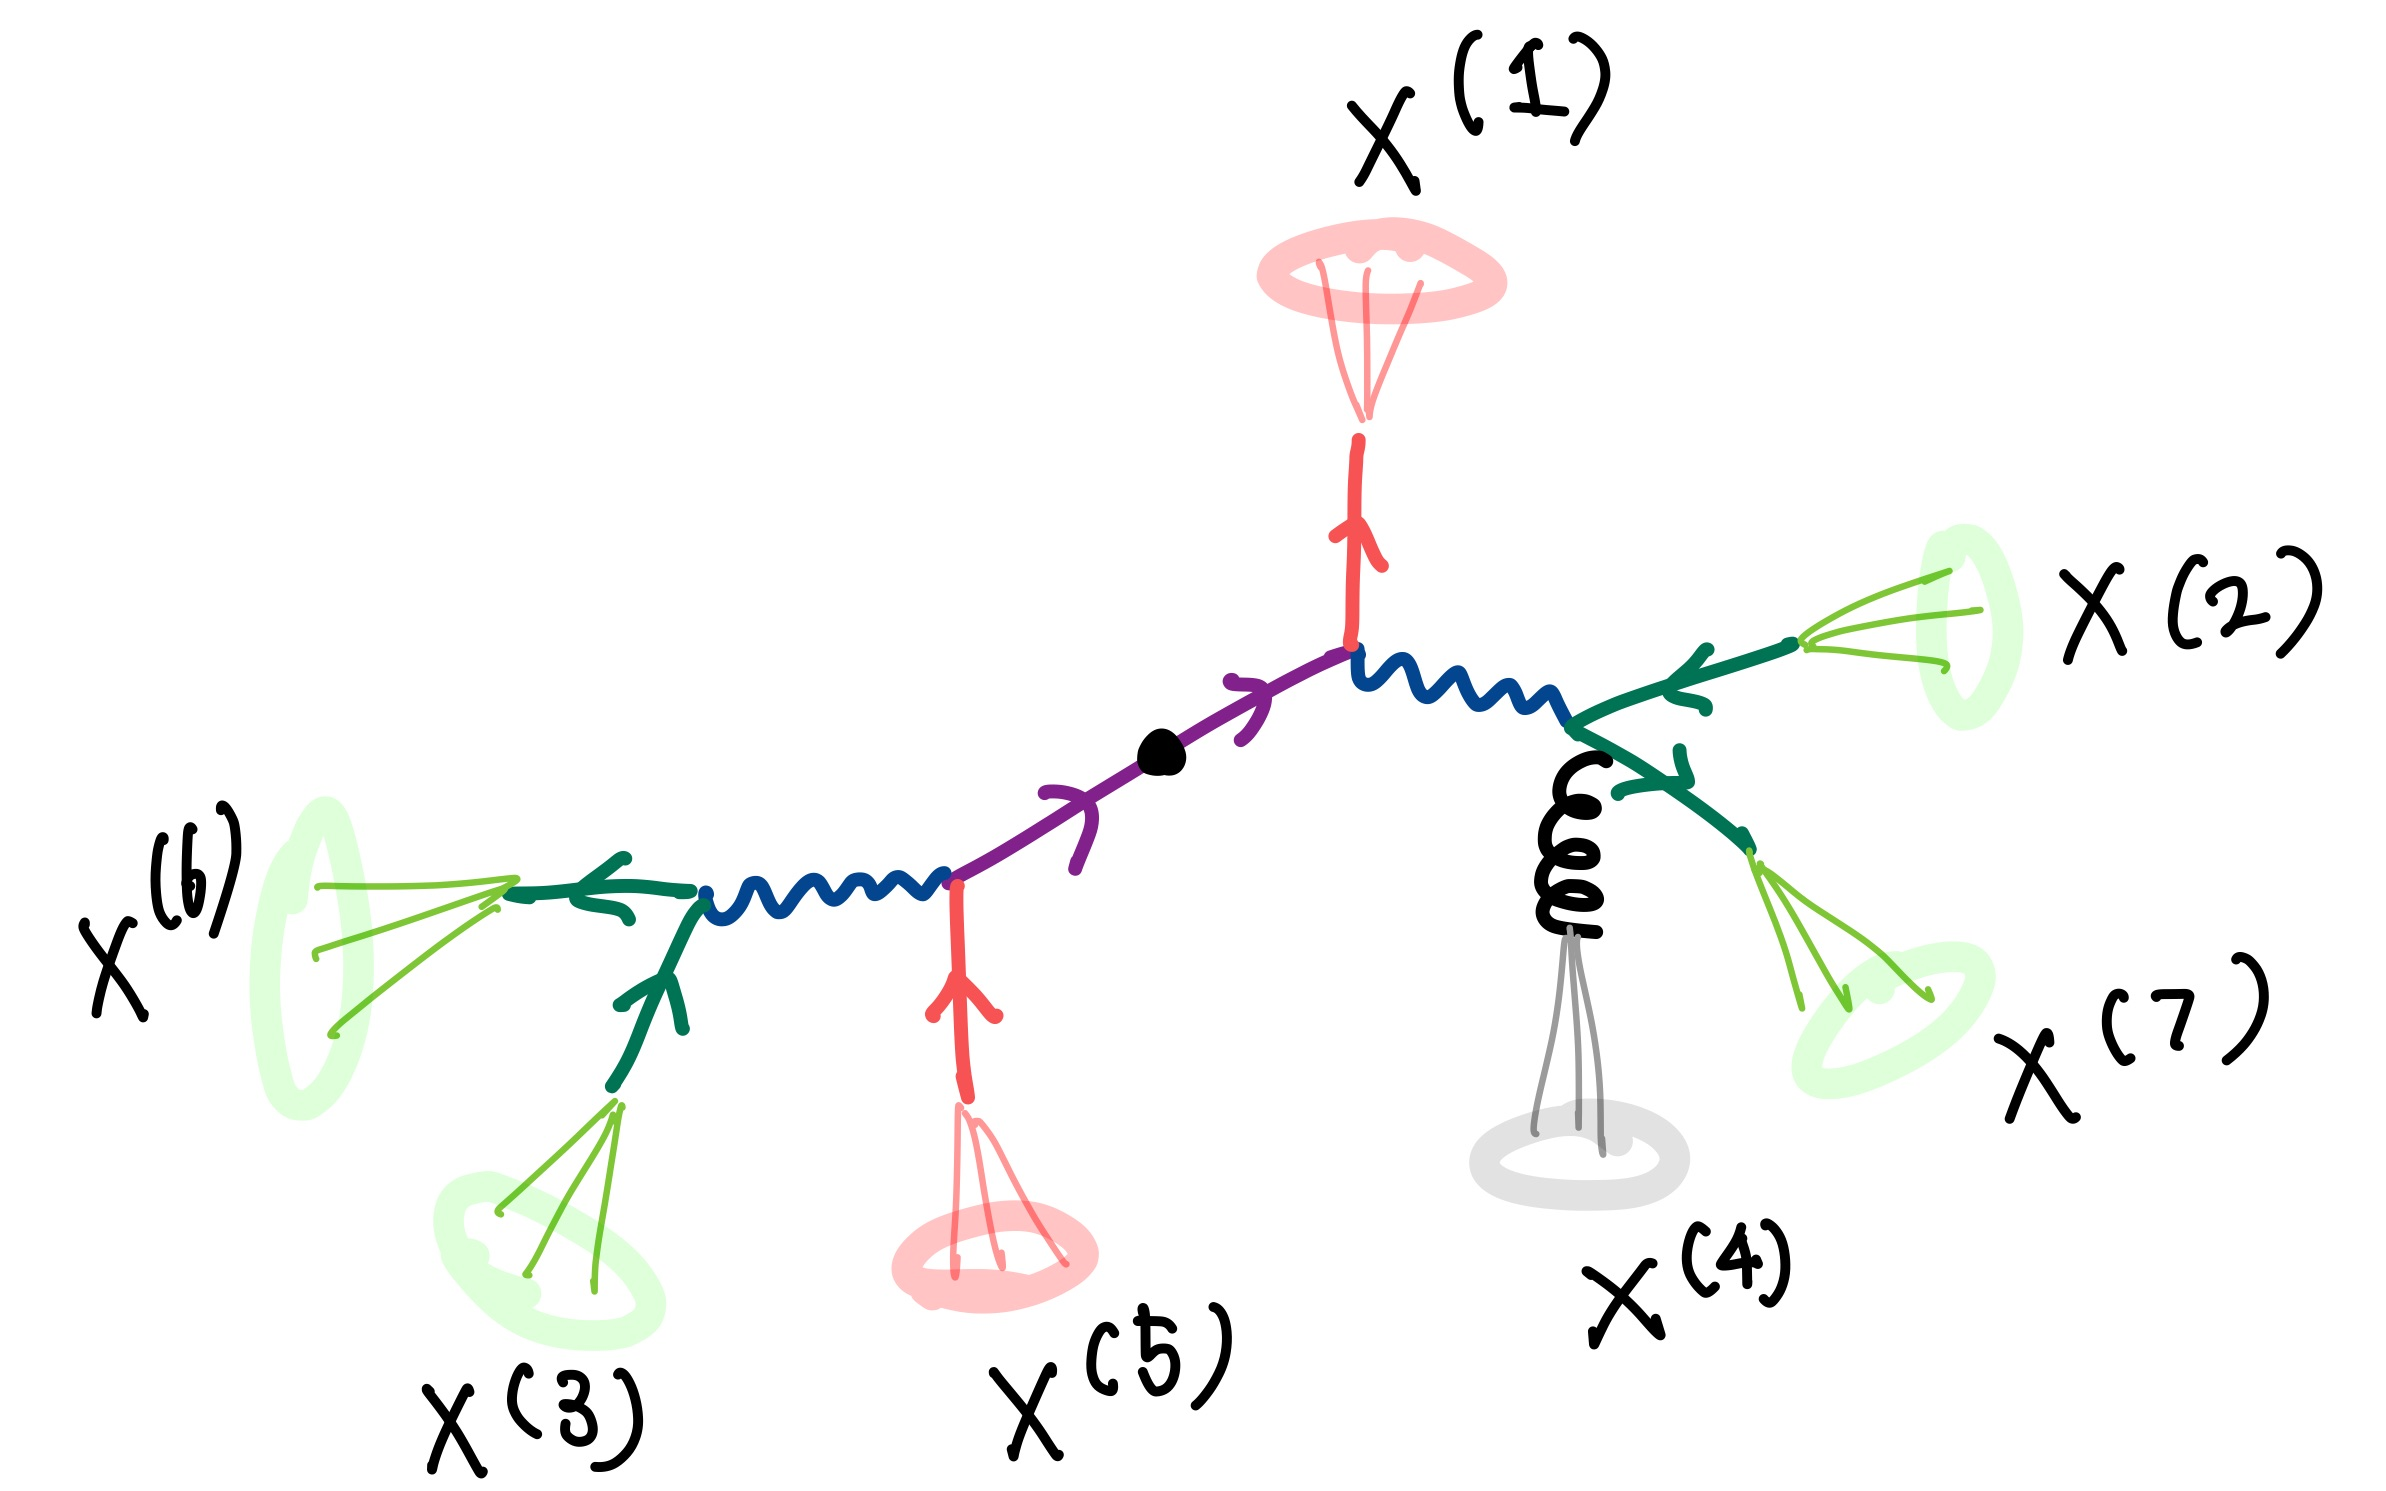
\includegraphics[width=0.3\textwidth]{figures/misc/saja-input.jpg}
        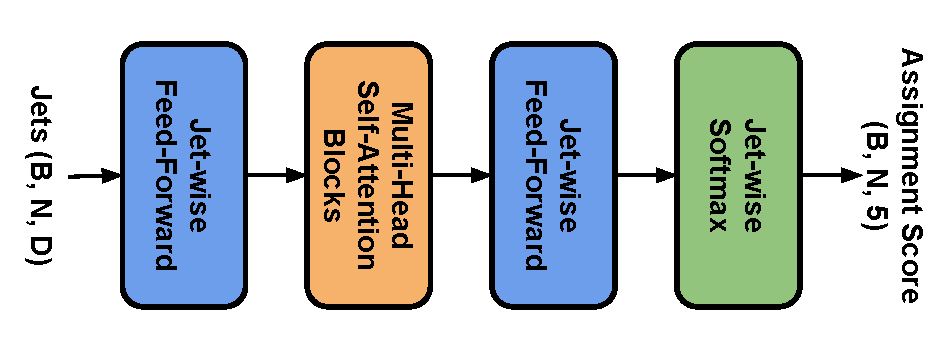
\includegraphics[width=0.3\textwidth]{figures/model/model-rot270.pdf}
        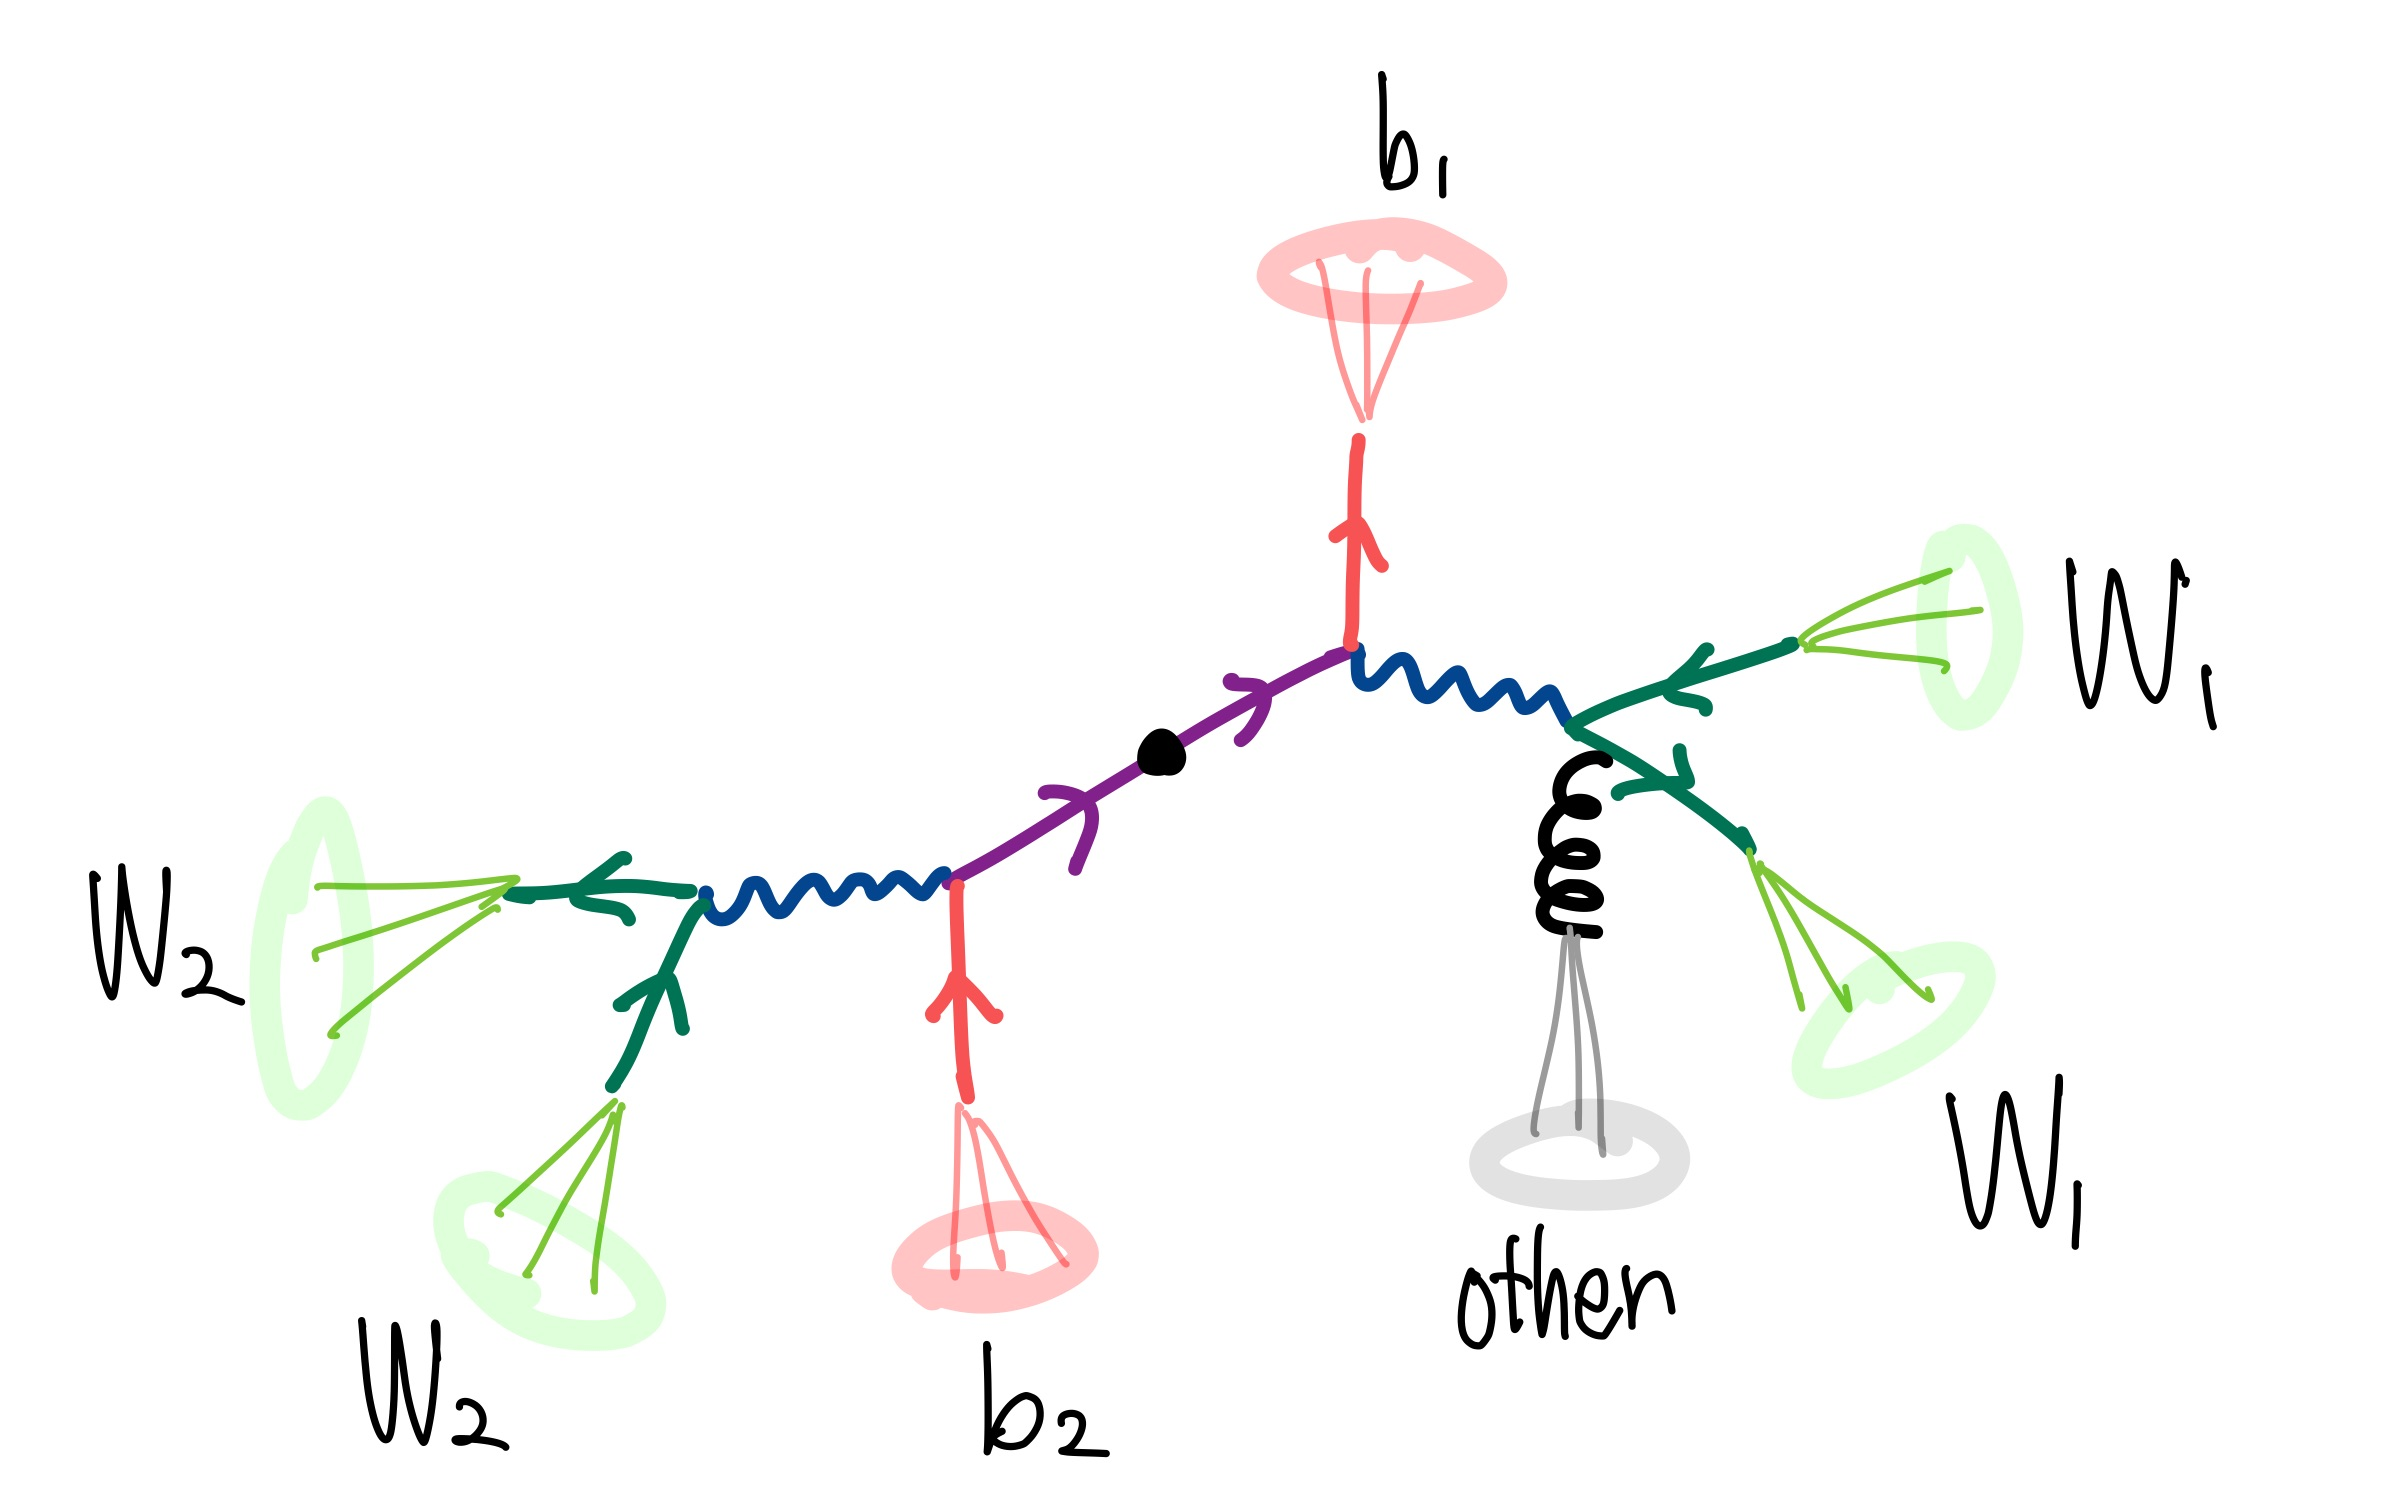
\includegraphics[width=0.3\textwidth]{figures/misc/saja-output.jpg}
    \end{figure}


\end{frame}



%%%%%%%%%%%%%%%%%%%%%%%%%%%%%%%%%%%%%%%%%%%%%%%%%%%%%%%%%%%%%%%%%%%%%%%%%%%%%%%%


\begin{frame}[fragile]{Objective function}
    Since the indices 1 and 2 are arbitrary, the general objective function cannot be used here. \break
    Therefore, a new cross-entropy based objective function is introduced.
    \begin{gather*}
        J(\theta) = \frac{1}{N} \sum_{j=1}^{N}[\min{(\pi_{12}^{(j)}, \pi_{21}^{(j)})} + y_{ \textrm{other} }^{(j)} \log{\hat{y}_{\textrm{other}}^{(j)}}],
        \intertext{where}
        \pi_{\alpha\beta}^{(j)} = -\left[
            y_{b}^{(j)} \log{\hat{y}_{b_{\alpha}}^{(j)}}
            + y_{\bar{b}}^{(j)} \log{\hat{y}_{b_{\beta}}^{(j)}} 
            + y_{W^{+}}^{(j)} \log{\hat{y}_{W_{\alpha}}^{(j)}}
            + y_{W^{-}}^{(j)} \log{\hat{y}_{W_{\beta}}^{(j)}}
            \right].
    \end{gather*}
    
    $\Rightarrow$ A deep learning model of any architecture can become a \underline{\textbf{zero-permutation jet-parton assignment model}} if it is fit by minimizing the above objective function.
\end{frame}





%%%%%%%%%%%%%%%%%%%%%%%%%%%%%%%%%%%%%%%%%%%%%%%%%%%%%%%%%%%%%%%%%%%%%%%%%%%%%%%%
%%%%%%%%%%%%%%%%%%%%%%%%%%%%%%%%%%%%%%%%%%%%%%%%%%%%%%%%%%%%%%%%%%%%%%%%%%%%%%%%

%\section[Attention Mechanism]{Attention Mechanism}

\begin{frame}[fragile]{Self-Attention based Model Architecture}

    $\bullet$ The model implementation is based on \textsc{Transformer}, which is the neural machine translation model and features \underline{\textbf{self-attention}}. \href{https://arxiv.org/abs/1706.03762}{[A. Vaswani, arXiv:1706.03762]}
    
    $\bullet$ Self-attention performs a weight sum of the elements (vectors) of the input set, where the weight matrix is also computed from the elements.
        \begin{itemize}
            \item Sequence = a set of words
            \item Image = a set of pixels
            \item Event = a set of jets
        \end{itemize}
    
    $\bullet$ Self-attention based model can learn the dependency between elements.
    \bigskip

\end{frame}


\begin{frame}[fragile]{Scaled Dot-Product Attention (0)}
    \begin{columns}
        \column{0.3\textwidth}
        \begin{figure}
            \centering
            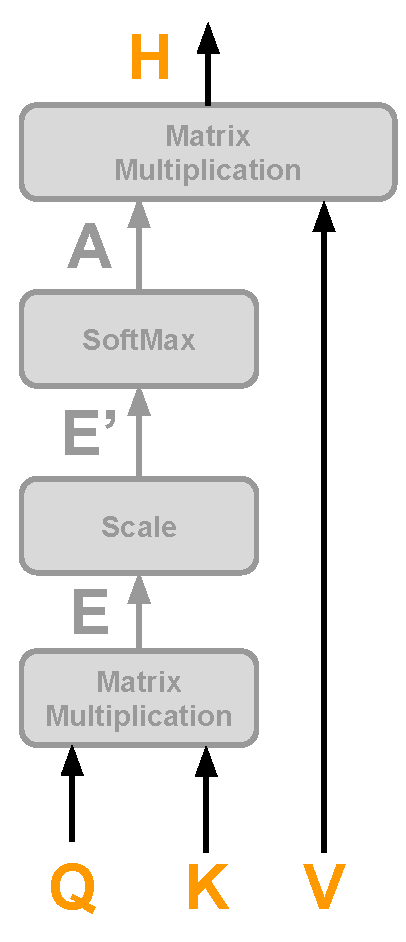
\includegraphics[width=\textwidth]{figures/model/attention_step0-type2.pdf}
            %\caption{Caption}
            %\label{fig:my_label}
        \end{figure}

        \column{0.55\textwidth}
        {\footnotesize $\bullet$ The set is represented as the matrix.}
        \begin{flalign*}
            \footnotesize
           X = \begin{bmatrix}
                    \vec{x}_{1} \\
                    \vec{x}_{2} \\
                    \vec{x}_{3}
                \end{bmatrix}
        \end{flalign*}
        {\footnotesize $\bullet$ Attention function takes three sets K, V and Q as input and produces a set. In general, K and V are originated from the same set X.}
        \begin{flalign*}
            \tiny H &= Attention(K,V,Q) \\
                    &= Attention(\phi_{K}(X), \phi_{V}(X), Q)
        \end{flalign*}
        {\footnotesize $\bullet$ Self-Attention is a special case of attention, where Q is also came from X.}
    \end{columns}
\end{frame}


\begin{frame}[fragile]{Scaled Dot-Product Attention (1)}
    \begin{columns}
        \column{0.3\textwidth}
        \begin{figure}
            \centering
            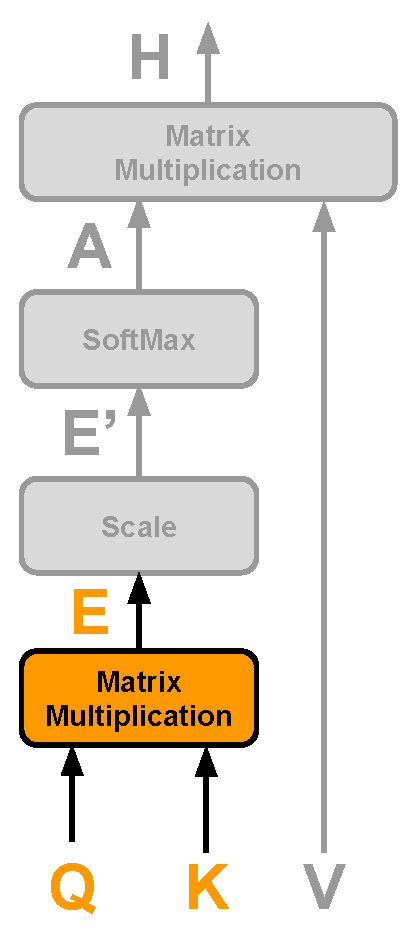
\includegraphics[width=\textwidth]{figures/model/attention_step1.pdf}
            %\caption{Caption}
            %\label{fig:my_label}
        \end{figure}

        \column{0.55\textwidth}
        \begin{flalign*}
            E &= Q K^{T} \\
              &= \begin{bmatrix}
                    {\color{orange}  \vec{q}_{1}} \\
                    \vec{q}_{2} \\
                    \vec{q}_{3}
                \end{bmatrix}
                \begin{bmatrix}
                    \vec{k}_{1} & {\color{orange} \vec{k}_{2}} & \vec{k}_{3}
                \end{bmatrix} \\
             &=  \begin{bmatrix}
                    \vec{q}_{1}\cdot\vec{k}_{1} & {\color{orange} \vec{q}_{1}\cdot\vec{k}_{2}} & \vec{q}_{1}\cdot\vec{k}_{3} \\
                    \vec{q}_{2}\cdot\vec{k}_{1} & \vec{q}_{2}\cdot\vec{k}_{2} & \vec{q}_{2}\cdot\vec{k}_{3} \\
                    \vec{q}_{3}\cdot\vec{k}_{1} & \vec{q}_{3}\cdot\vec{k}_{2} & \vec{q}_{3}\cdot\vec{k}_{3}
                \end{bmatrix}.
        \end{flalign*}
    \end{columns}
\end{frame}


\begin{frame}[fragile]{Scaled Dot-Product Attention (2)}
    \begin{columns}
        \column{0.3\textwidth}
        \begin{figure}
            \centering
            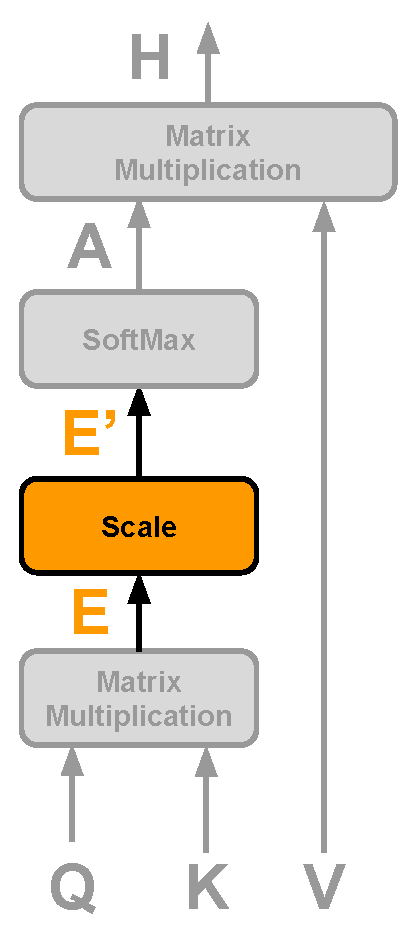
\includegraphics[width=\textwidth]{figures/model/attention_step2.pdf}
            %\caption{Caption}
            %\label{fig:my_label}
        \end{figure}

        \column{0.55\textwidth}
        \begin{flalign*}
            E &= Q K^{T} \\
              &= \begin{bmatrix}
                    \vec{q}_{1} \\
                    \vec{q}_{2} \\
                    \vec{q}_{3}
                \end{bmatrix}
                \begin{bmatrix}
                    \vec{k}_{1} & \vec{k}_{2}& \vec{k}_{3}
                \end{bmatrix} \\
             &=  \begin{bmatrix}
                    \vec{q}_{1}\cdot\vec{k}_{1} & \vec{q}_{1}\cdot\vec{k}_{2} & \vec{q}_{1}\cdot\vec{k}_{3} \\
                    \vec{q}_{2}\cdot\vec{k}_{1} & \vec{q}_{2}\cdot\vec{k}_{2} & \vec{q}_{2}\cdot\vec{k}_{3} \\
                    \vec{q}_{3}\cdot\vec{k}_{1} & \vec{q}_{3}\cdot\vec{k}_{2} & \vec{q}_{3}\cdot\vec{k}_{3}
                \end{bmatrix}. \\
            E' &=  \frac{1}{\sqrt{{\color{orange}dim({\vec{k}})}}}E.
        \end{flalign*}
    \end{columns}
\end{frame}


\begin{frame}[fragile]{Scaled Dot-Product Attention (3)}
    \begin{columns}
        \column{0.3\textwidth}
        \begin{figure}
            \centering
            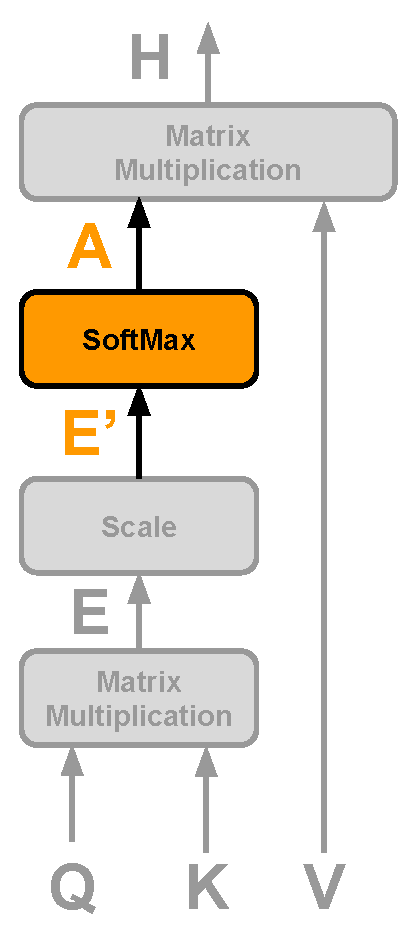
\includegraphics[width=\textwidth]{figures/model/attention_step3.pdf}
            %\caption{Caption}
            %\label{fig:my_label}
        \end{figure}

        \column{0.55\textwidth}
        \begin{flalign*}
            \Large
            A = \begin{bmatrix}
                    \frac{ e^{E'_{\textcolor{orange}{1}1}} }{ Z_{\textcolor{orange}{1}} } & \frac{ e^{E'_{\textcolor{orange}{1}2}} }{ Z_{\textcolor{orange}{1}} } & \frac{ e^{E'_{\textcolor{orange}{1}3}} }{ Z_{\textcolor{orange}{1}} } \\
                    \frac{ e^{E'_{21}} }{ Z_{2} } & \frac{ e^{E'_{22}} }{ Z_{2} } & \frac{ e^{E'_{23}} }{ Z_{2} } \\
                    \frac{ e^{E'_{31}} }{ Z_{3} } & \frac{ e^{E'_{32}} }{ Z_{3} } & \frac{ e^{E'_{33}} }{ Z_{3} }
                \end{bmatrix},
            \intertext{where $Z_{j}=\sum_{j}e^{E'_{ij}}$.}
        \end{flalign*}
        
    \end{columns}
\end{frame}

\begin{frame}[fragile]{Scaled Dot-Product Attention (4)}
    \begin{columns}
        \column{0.3\textwidth}
        \begin{figure}
            \centering
            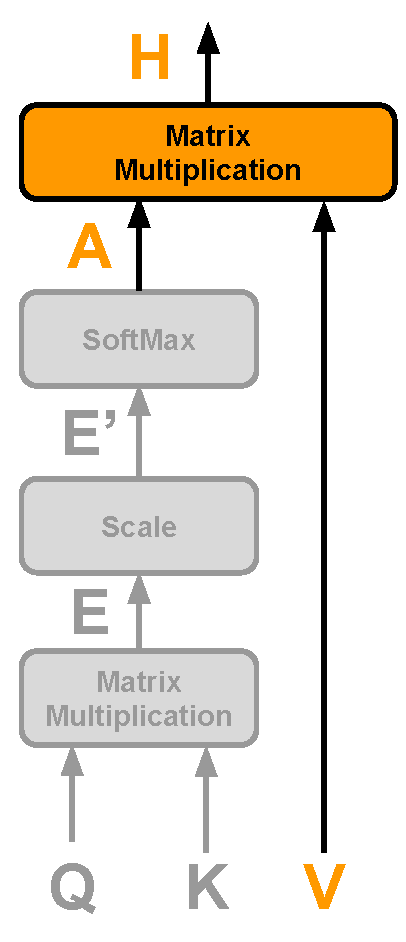
\includegraphics[width=\textwidth]{figures/model/attention_step4.pdf}
            %\caption{Caption}
            %\label{fig:my_label}
        \end{figure}

        \column{0.65\textwidth}

        \begin{flalign*}
            \Large
            H &= \begin{bmatrix}
                    \textcolor{orange}{A_{11}} & \textcolor{orange}{A_{12}} & \textcolor{orange}{A_{13}} \\
                    A_{21} & A_{22} & A_{23} \\
                    A_{31} & A_{32} & A_{33}
                 \end{bmatrix}
                 \begin{bmatrix}
                    \textcolor{orange}{\vec{v}_{1}} \\
                    \textcolor{orange}{\vec{v}_{2}} \\
                    \textcolor{orange}{\vec{v}_{3}}
                 \end{bmatrix} \\
              &= \begin{bmatrix}
                    \textcolor{orange}{\sum_{i} A_{1i} \vec{v}_{i}} \\
                    \sum_{i} A_{2i} \vec{v}_{i} \\
                    \sum_{i} A_{3i} \vec{v}_{i}
                 \end{bmatrix}.
        \end{flalign*}
    \end{columns}
\end{frame}



\begin{frame}[fragile]{Multi-head Attention}
    \begin{figure}
        \centering
        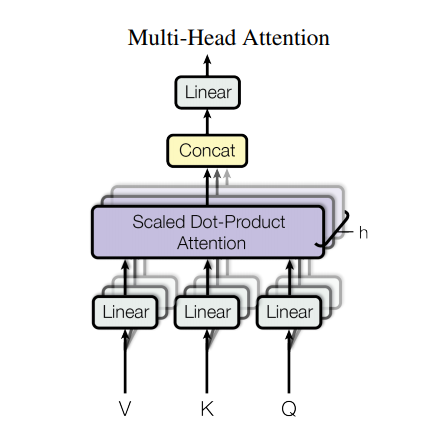
\includegraphics[width=0.5\textwidth]{figures/model/multi_head_attention.png}
    \end{figure}
    Multi-Head Attention consists of several attention layers running in parallel. Reprinted from "Attention Is All You Need" \href{https://arxiv.org/abs/1706.03762}{[arXiv:1706.03762]}
\end{frame}

%%%%%%%%%%%%%%%%%%%%%%%%%%%%%%%%%%%%%%%%%%%%%%%%%%%%%%%%%%%%%%%%%%%%%%%%%%%%%%%%
\begin{frame}[fragile]{Self-Attention based Model Architecture $(\textsc{SaJa})$}
    \begin{figure}
        \centering
        \begin{subfigure}[t]{0.3\textwidth}
            \centering
            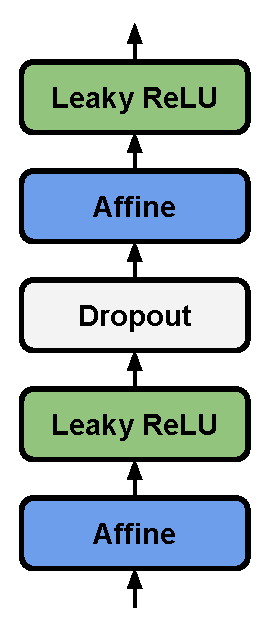
\includegraphics[width=\textwidth, height=5cm, keepaspectratio]{figures/model/jet-wise-feed-forward.pdf}
            \caption{Jet-wise feed-forward network}
        \end{subfigure}
        \hfill  
        \begin{subfigure}[t]{0.3\textwidth}
            \centering
            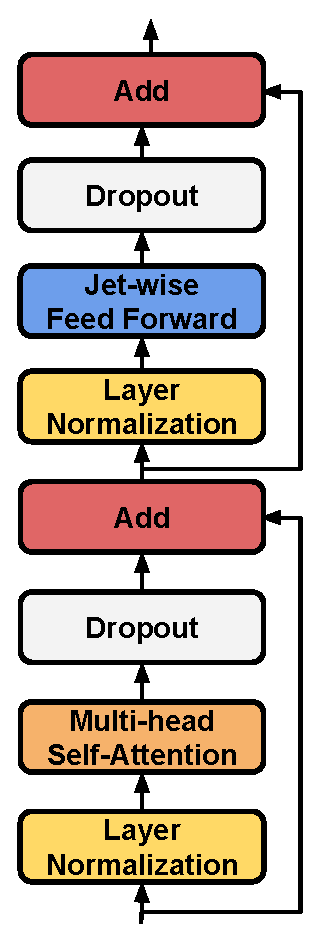
\includegraphics[width=\textwidth, height=6cm, keepaspectratio]{figures/model/attention-block.pdf}
            \caption{Multi-head self-attention block}
        \end{subfigure}
        \hfill
        \begin{subfigure}[t]{0.3\textwidth}
            \centering
            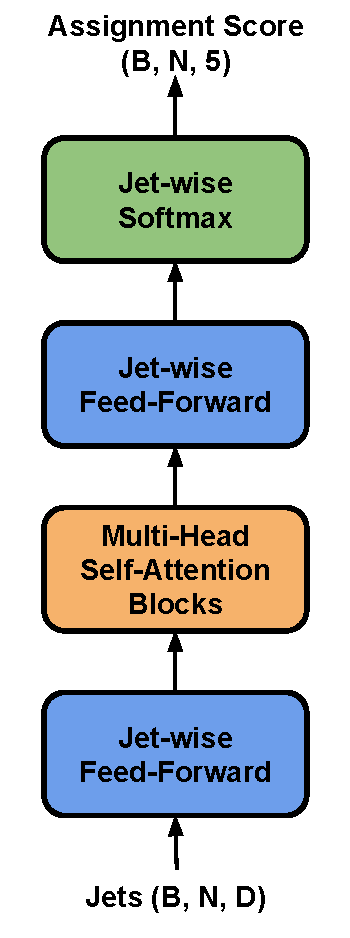
\includegraphics[width=\textwidth, height=5cm, keepaspectratio]{figures/model/model.pdf}
            \caption{\saja, Jet-parton assignment model}
        \end{subfigure}
      \hfill
      %\caption{\label{fig:architecture} \(B\) denotes the batch size. \(N\) indicates the maximum number of jets in the batch. \(D\) indicates the number of features representing the jet.}
    \end{figure}
    {\footnotesize \saja\, is invariant to the order of jets and this permutation invariant property can be used to peek inside the black box of \saja\, with Monte Carlo information.}
\end{frame}


%%%%%%%%%%%%%%%%%%%%%%%%%%%%%%%%%%%%%%%%%%%%%%%%%%%%%%%%%%%%%%%%%%%%%%%%%%%%%%%%
%\section{Simulated Dataset}
\begin{frame}[fragile]{Simulation}
    \begin{block}{$\blacksquare$ Generation}
        \smallskip
        \begin{itemize}
            \item pp collision with $\sqrt{s}=13\,\text{TeV}$ using $\textsc{MadGraph5\_aMC@NLO}$ and $\textsc{Pythia8}$
            \item Fully hadronic $ t\bar{t} $ with up to two additional jets at NLO, $m_{t}=172.5\,\textGeV$
            \item QCD multijet at LO.
        \end{itemize}
    \end{block}
    \medskip
    \begin{block}{$\blacksquare$ Detector response}
        \smallskip
        \begin{itemize}
            \item \textsc{Delphes3}
            \item CMS-like detector
        \end{itemize}
    \end{block}
    \begin{block}{$\blacksquare$ Jet Finding}
        \smallskip
        \begin{itemize}
            \item \textsc{FastJet3}
            \item anti-$k_{T}$ algorithm with R=0.4
        \end{itemize}
    \end{block}
\end{frame}


%%%%%%%%%%%%%%%%%%%%%%%%%%%%%%%%%%%%%%%%%%%%%%%%%%%%%%%%%%%%%%%%%%%%%%%%%%%%%%%%
\begin{frame}[fragile]{Selection}

    Selection follows the trigger selection used in the CMS $t\bar{t}$ all-jets analysis. {\scriptsize \href{https://link.springer.com/article/10.1140\%2Fepjc\%2Fs10052-019-6788-2}{[CMS, Eur. Phys. J. C 79 (2019) 313]}}.

    \begin{columns}[T,onlytextwidth]
        \column{\textwidth}
        \begin{block}{$\blacksquare$ Jet}
            \begin{itemize}
                \item $ p_{T} \textgreater 30\,\textGeV $
                \item $ \abs{\eta} \textless 2.4 $
                \item[+]  b-tag: true/fake based on the efficiency for b quark and misidentification rates for gluon, light quark jets and c-jets.
            \end{itemize}
        \end{block}
        
        \begin{block}{$\blacksquare$ Event}
            \begin{itemize}
                \item $N_{\text{jet}} \ge 6$
                %\item $N_{\text{b-tagged jet}} \ge 1$
                \item At least one b-tagged jet of the six most energetic jets
                \item $p_{T}(\text{jet}_{6}) \textgreater 40\,\textGeV$
                \item $H_{T} \equiv \sum_{\textjet} p_{T} \textgreater 450\,\textGeV$
            \end{itemize}
        \end{block}


    \end{columns}
\end{frame}


\begin{frame}[fragile]{Jet-Parton Matching}
    After the event selection, only about 20\% of $t\bar{t}$ events satisfy the following jet-parton matching condition and are called \textbf{matched}.
    $$\Delta R(\text{jet}, \text{parton}) = \sqrt{\Delta\eta^{2}+\Delta\phi^{2}} < 0.3$$
    Only the matched $t\bar{t}$ events are used to train the DL model.
    \begin{columns}[T,onlytextwidth]
        \column{0.48\textwidth}
        \begin{figure}
            \centering
            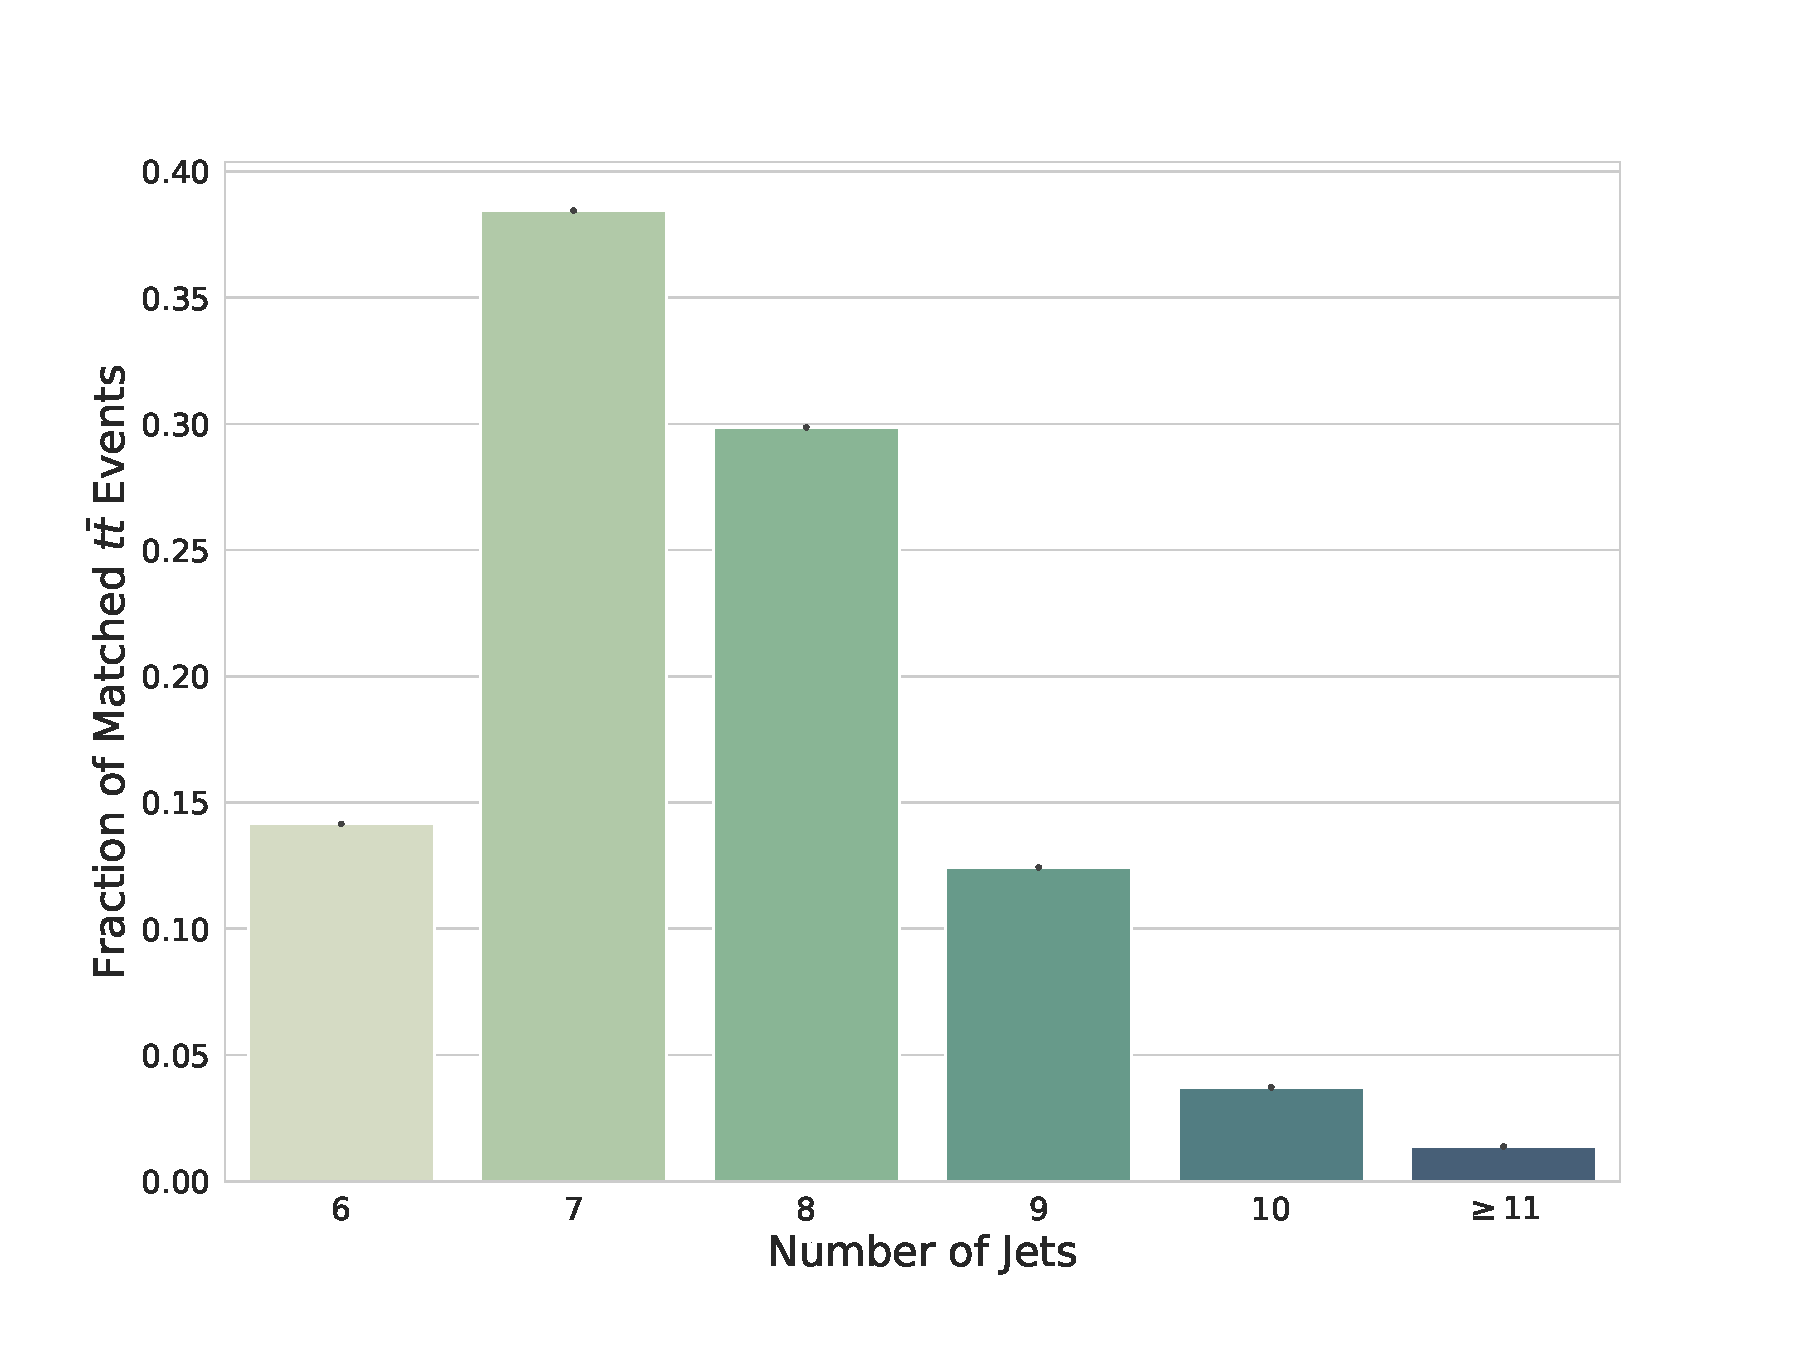
\includegraphics[width=0.8\textwidth]{figures/misc/num-jets.pdf}
            \caption{The distribution of the number of jets in the matched $t\bar{t}$ events}
        \end{figure}
        \column{0.48\textwidth}
        \begin{figure}
            \centering
            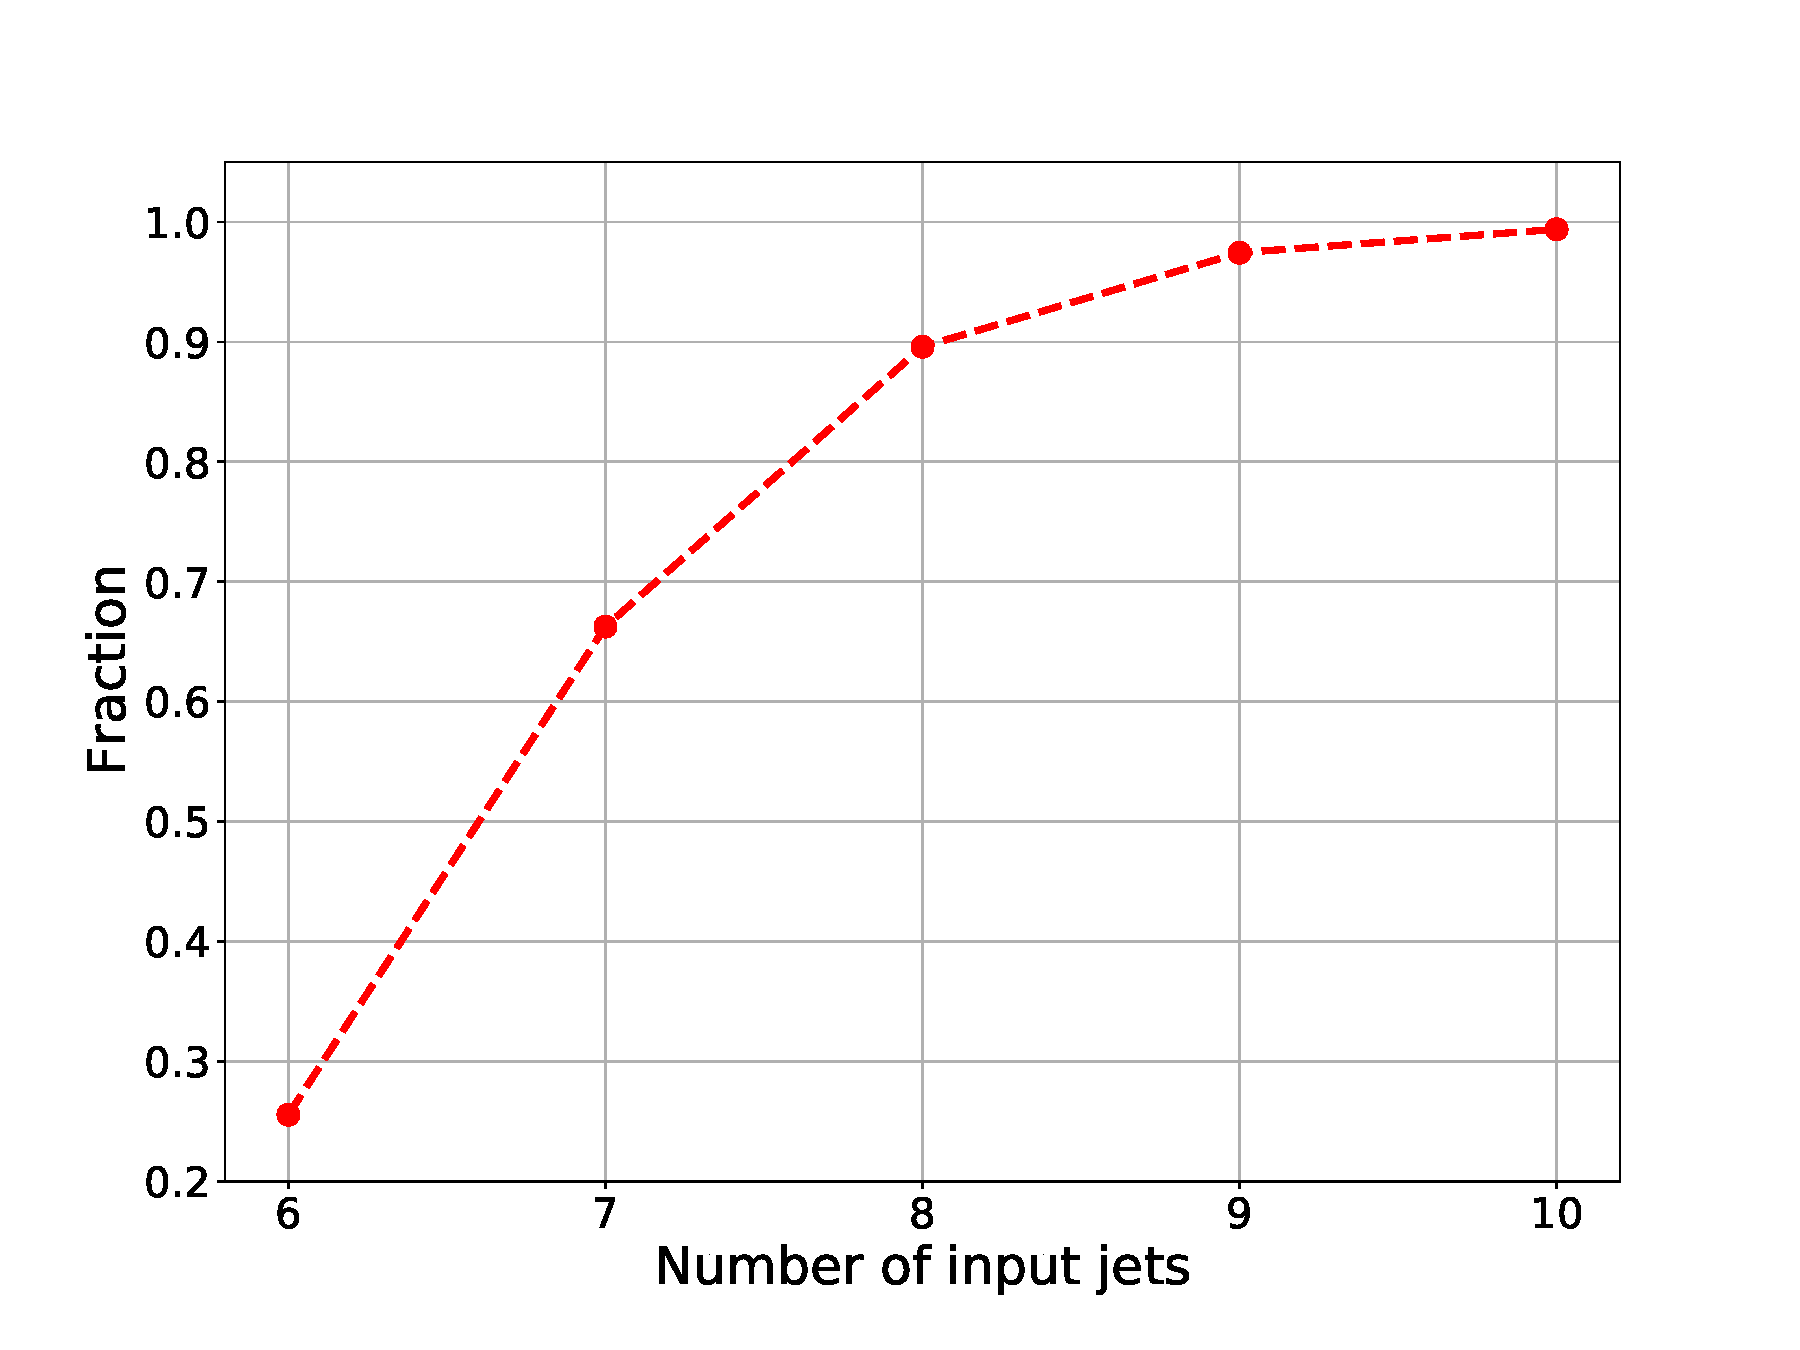
\includegraphics[width=0.8\textwidth]{figures/misc/frac-vs-num-jets.pdf}
            \caption{The fraction of matched $t\bar{t}$ events, where all partons can be matched with the most energetic $N$ jets.}
            %\label{fig:my_label}
        \end{figure}
    \end{columns}
\end{frame}



%%%%%%%%%%%%%%%%%%%%%%%%%%%%%%%%%%%%%%%%%%%%%%%%%%%%%%%%%%%%%%%%%%%%%%%%%%%%%%%%

\begin{frame}[fragile]{Training Dataset}
    \begin{block}{$\blacksquare$ Event}
        \smallskip
        All jets in the event are used as input to the model.
        
        For simplicity, the jet is high level reconstructed variables.
        $$\footnotesize (p_{T}, \eta, \phi, \frac{p_{T}}{H_{T}}, \text{b-tag})$$
    \end{block}
    \begin{block}{$\blacksquare$ Jet Shape}
        %\smallskip
        Gluon-initiated jets should always be assigned to $'\text{other}'$. So the effect of the following jet shape variables is studied.
        \href{https://arxiv.org/abs/1409.3072}{[CMS, arXiv:1409.3072]}
        \begin{itemize}
            \item {\footnotesize $p_{T}D=\frac{ \sum_{i} p_{T,i}^{2} }{ \sum_{i} p_{T,i} }$}
            \item {\footnotesize Major and minor axes of the jet axis in $\eta-\phi$ space}
            \item {\footnotesize Charged hadron, neutral hadron, electrons, muon, and photon multiplicities}
        \end{itemize}
    \end{block}
    \begin{block}{$\blacksquare$ Pre-processing}
        %\smallskip
        {\footnotesize All features except b-tag is scaled to [0, 1] through min-max scaling $x'=\frac{x-\min({x})}{\max({x})-\min({x})}$}
    \end{block}
    
\end{frame}


%%%%%%%%%%%%%%%%%%%%%%%%%%%%%%%%%%%%%%%%%%%%%%%%%%%%%%%%%%%%%%%%%%%%%%%%%%%%%%%%
%%%%%%%%%%%%%%%%%%%%%%%%%%%%%%%%%%%%%%%%%%%%%%%%%%%%%%%%%%%%%%%%%%%%%%%%%%%%%%%%
%%%%%%%%%%%%%%%%%%%%%%%%%%%%%%%%%%%%%%%%%%%%%%%%%%%%%%%%%%%%%%%%%%%%%%%%%%%%%%%%
%\section{Training}





%%%%%%%%%%%%%%%%%%%%%%%%%%%%%%%%%%%%%%%%%%%%%%%%%%%%%%%%%%%%%%%%%%%%%%%%%%%%%%%%

%\begin{frame}[fragile]{Training details}
%    \begin{itemize}
%        \item Training, validation, test set: 300k, 80k, 100k events
%        \item Adam optimization
%        \item Learning rate schedule, which reduces the learning rate when the metric on the validation set has stopped improving.
%        \item PyTorch 1.3
%    \end{itemize}
%\end{frame}


%%%%%%%%%%%%%%%%%%%%%%%%%%%%%%%%%%%%%%%%%%%%%%%%%%%%%%%%%%%%%%%%%%%%%%%%%%%%%%%%

\begin{frame}[fragile]{Predictive Entropy}
    \metroset{block=fill}
    \begin{alertblock}{NB}
        {\footnotesize In this slides, the uncertainty is ML-side terminology.}
    \end{alertblock}
    
    \begin{columns}[T,onlytextwidth]
        \column{0.65\textwidth}
        %If any of the predictions for the jets in the event is also wrong, the jet-parton assignment is wrong.\\

        $\bullet$ To suppress poor jet-parton assignments, the DL model uncertainty is studied.\\
        
        \medskip
        
        $\bullet$ The \textbf{predictive entropy} quantifies the uncertainty in the prediction of the classifier.
        \begin{equation*}
            H[\hat{Y}] = \frac{1}{N} \sum_{j=1}^{N} [ -\sum_{c \in \textrm{partons} } \hat{y}_{c}^{(j)} \log \hat{y}_{c}^{(j)} ]
        \end{equation*}
        
        $\bullet$ When the jet-parton assignment with the predictive entropy higher than the threshold, the event is not selected.

        + The uncertainty is also used to detect out-of-distribution test data (corresponding to QCD in this study).
        \column{0.3\textwidth}
        \begin{figure}
            \centering
            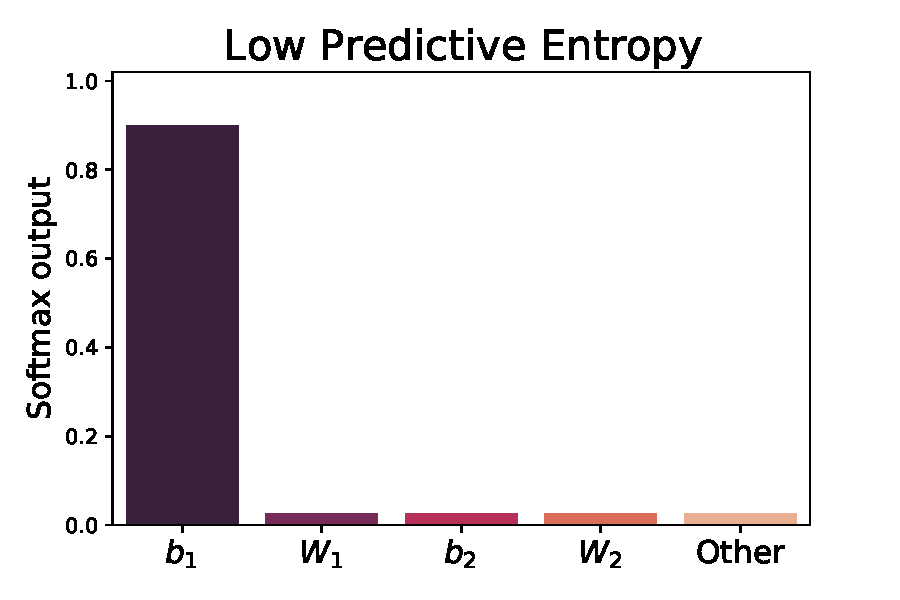
\includegraphics[width=\textwidth]{figures/misc/low-entropy.pdf}
            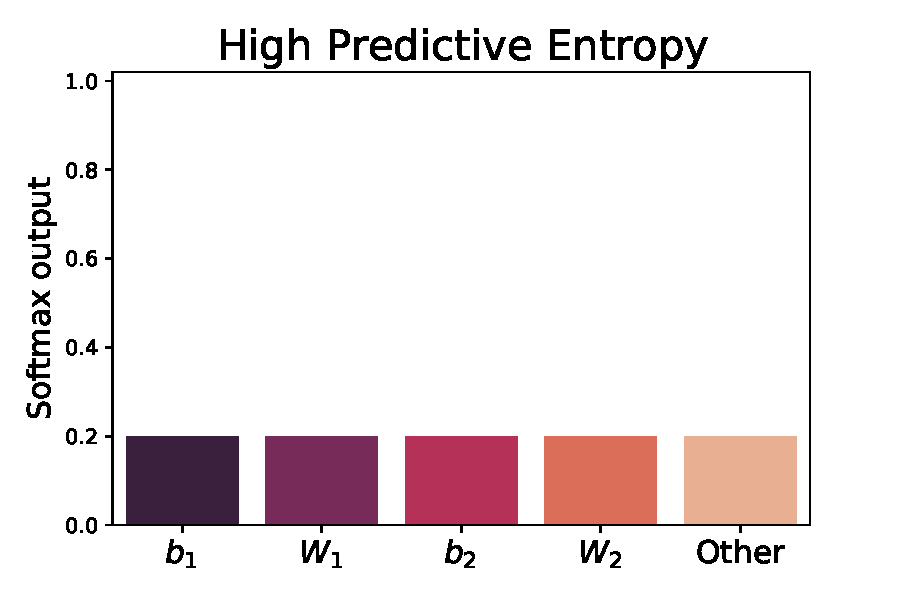
\includegraphics[width=\textwidth]{figures/misc/high-entropy.pdf}
            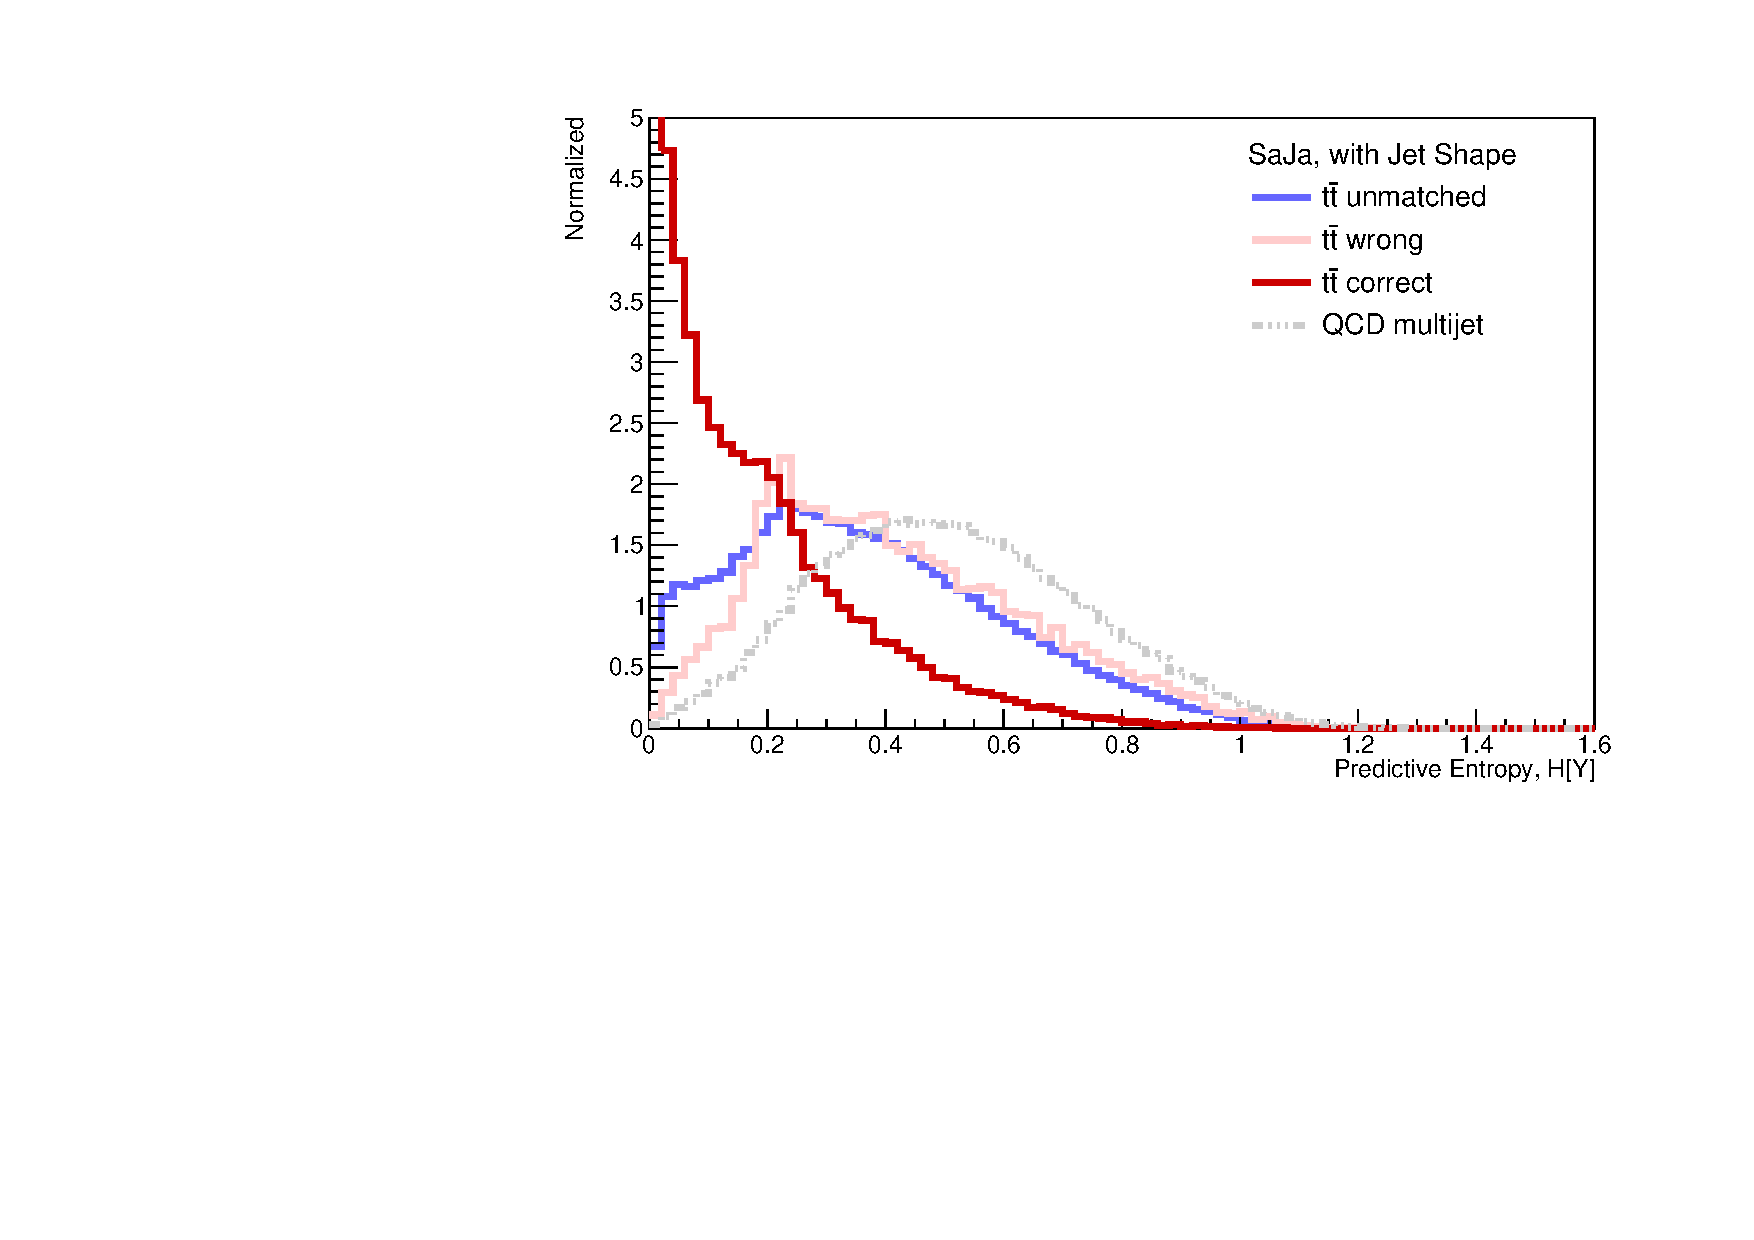
\includegraphics[width=\textwidth]{figures/entropy/entropy_with_jet_shape.pdf}
        \end{figure}
    \end{columns}
    
    
\end{frame}


%%%%%%%%%%%%%%%%%%%%%%%%%%%%%%%%%%%%%%%%%%%%%%%%%%%%%%%%%%%%%%%%%%%%%%%%%%%%%%%%
\begin{frame}[fragile]{Benchmark: Kinematic Likelihood Fitting}

    $\bullet$ Kinematic likelihood fitting is performed as a baseline study, the \href{https://github.com/KLFitter/KLFitter}{\textsc{KLFitter}} library is used. {\scriptsize \href{https://www.sciencedirect.com/science/article/pii/S0168900214001855?via\%3Dihub}{[J. Erdmann, Nucl.Instrum.Meth.A 748 (2014) 18-25]}}

    \scalebox{.7}{$
        \mathcal{L} = B(m_{q_{1}q_{2}q_{3}}|m_{t},\Gamma_{t}) \cdot
                     B(m_{q_{1}q_{2}}|m_{W},\Gamma_{W}) \cdot
                     B(m_{q_{4}q_{5}q_{6}}|m_{t},\Gamma_{t}) \cdot
                     B(m_{q_{4}q_{5}}|m_{W},\Gamma_{W}) \cdot
                     \prod_{i=1}^{6} W_{\text{jet}}(E_{\text{jet},i}^{\text{meas}}|E_{\text{jet},i})
    $},
    {\footnotesize where $B$ indicates the Breit-Wigner distribution and $W$ does the the transfer functions}
    
    %The \textsc{KLFitter} configuration used in \href{https://arxiv.org/pdf/1907.11181.pdf}{[J. Erdmann arXiv:1907.11181]} were followed.
    
    \smallskip
    
    $\bullet$ As more jets are used, the number of permutations increases explosively.
Therefore, two case are studied.
        \begin{itemize}
            \item[-] Most energetic 6 jets, $N_{jets}^{in} = 6 \rightarrow $ Avg. 18 permutations
            \item[-] Up to 7 most energetic jets $N_{jets}^{in} \leq 7 \rightarrow$  Avg. 126 permutations
        \end{itemize}
        
    \smallskip
    
    $\bullet$ When the best permutation has a likelihood lower than the threshold, the event is not selected.



\end{frame}

%%%%%%%%%%%%%%%%%%%%%%%%%%%%%%%%%%%%%%%%%%%%%%%%%%%%%%%%%%%%%%%%%%%%%%%%%%%%%%%%
%%%%%%%%%%%%%%%%%%%%%%%%%%%%%%%%%%%%%%%%%%%%%%%%%%%%%%%%%%%%%%%%%%%%%%%%%%%%%%%%
%%%%%%%%%%%%%%%%%%%%%%%%%%%%%%%%%%%%%%%%%%%%%%%%%%%%%%%%%%%%%%%%%%%%%%%%%%%%%%%%
%\section{Results}



%%%%%%%%%%%%%%%%%%%%%%%%%%%%%%%%%%%%%%%%%%%%%%%%%%%%%%%%%%%%%%%%%%%%%%%%%%%%%%%%

\begin{frame}[fragile]{Performance}

    \begin{columns}
        \column{0.55\textwidth}
        \medskip
        
        {\footnotesize $\bullet$ The assignment performance is visualized as ROC-like curves drawn by varying the threshold value for the predictive entropy of \textsc{SaJa} or the likelihood of \textsc{KLFitter}.}
        
        {\footnotesize $\bullet$  \textsc{SaJa} shows more powerful performance than \textsc{KLFitter}.}
        
        {\footnotesize $\bullet$ Predictive entropy not only reduces poor jet-parton assignments but also helps reduce unmatched $t\bar{t}$ and QCD multijet events without additional training process.}
        
        {\footnotesize $\bullet$  Jet shape increases the fraction of correct assignment.}
        
        \column{0.37\textwidth}
            \begin{figure}
            \centering
                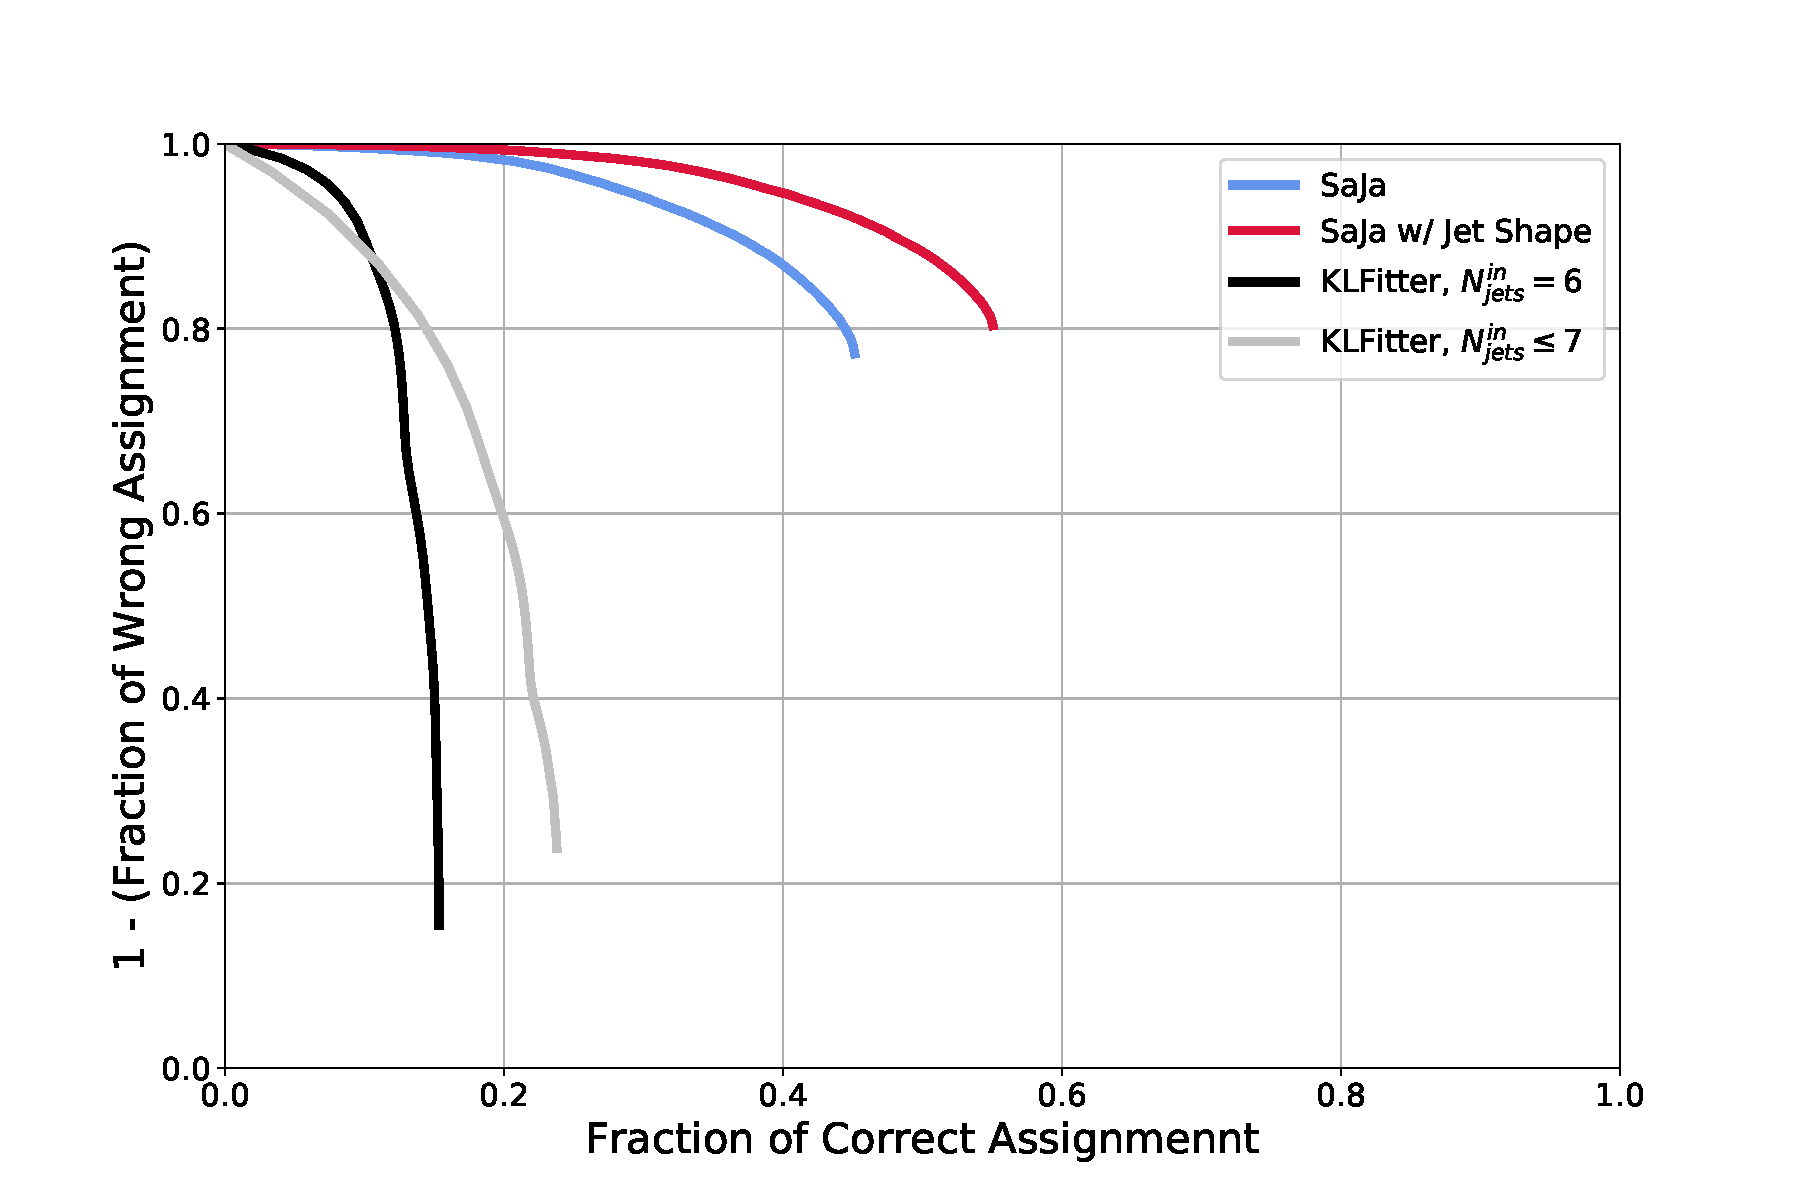
\includegraphics[width=\textwidth]{figures/roc/wrong_rej_vs_mat_tt_acc.pdf}
                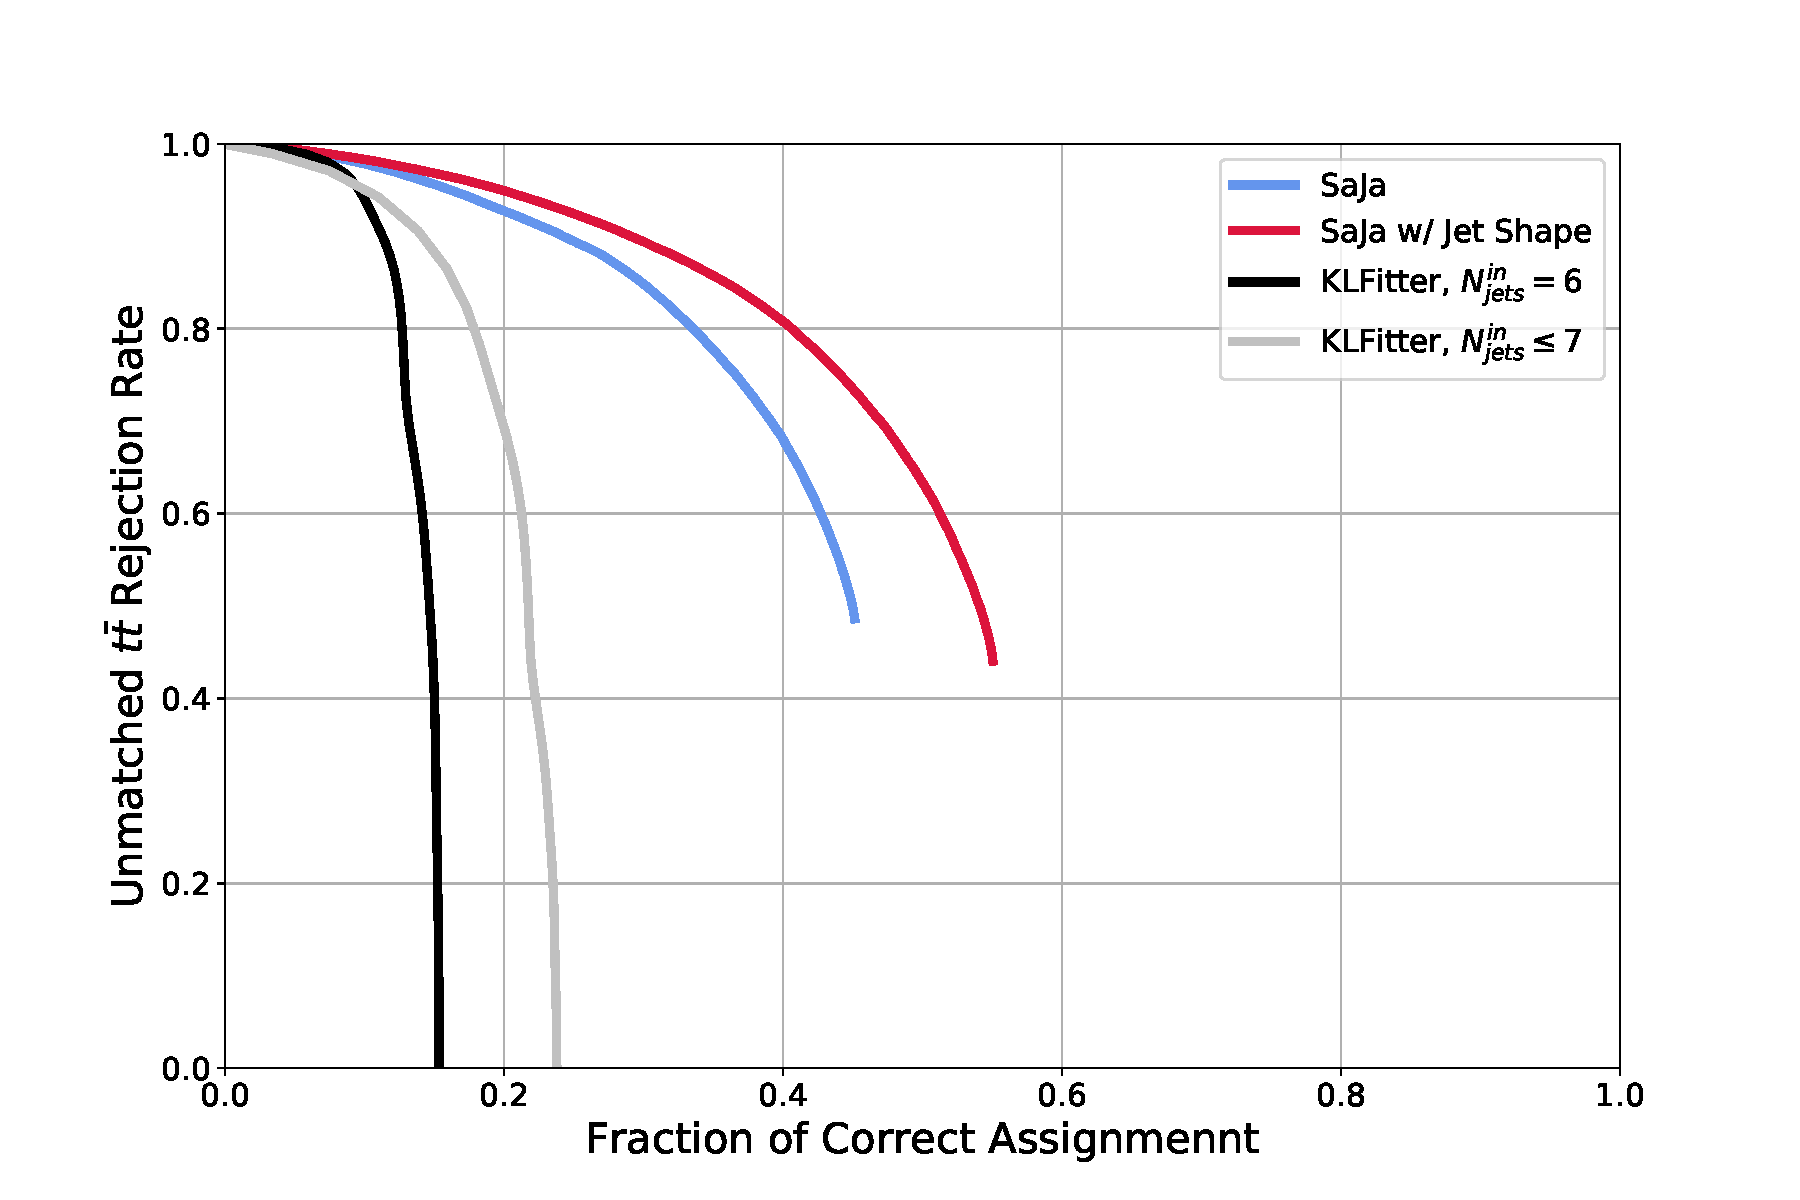
\includegraphics[width=\textwidth]{figures/roc/unmat_rej_vs_mat_tt_acc.pdf}
                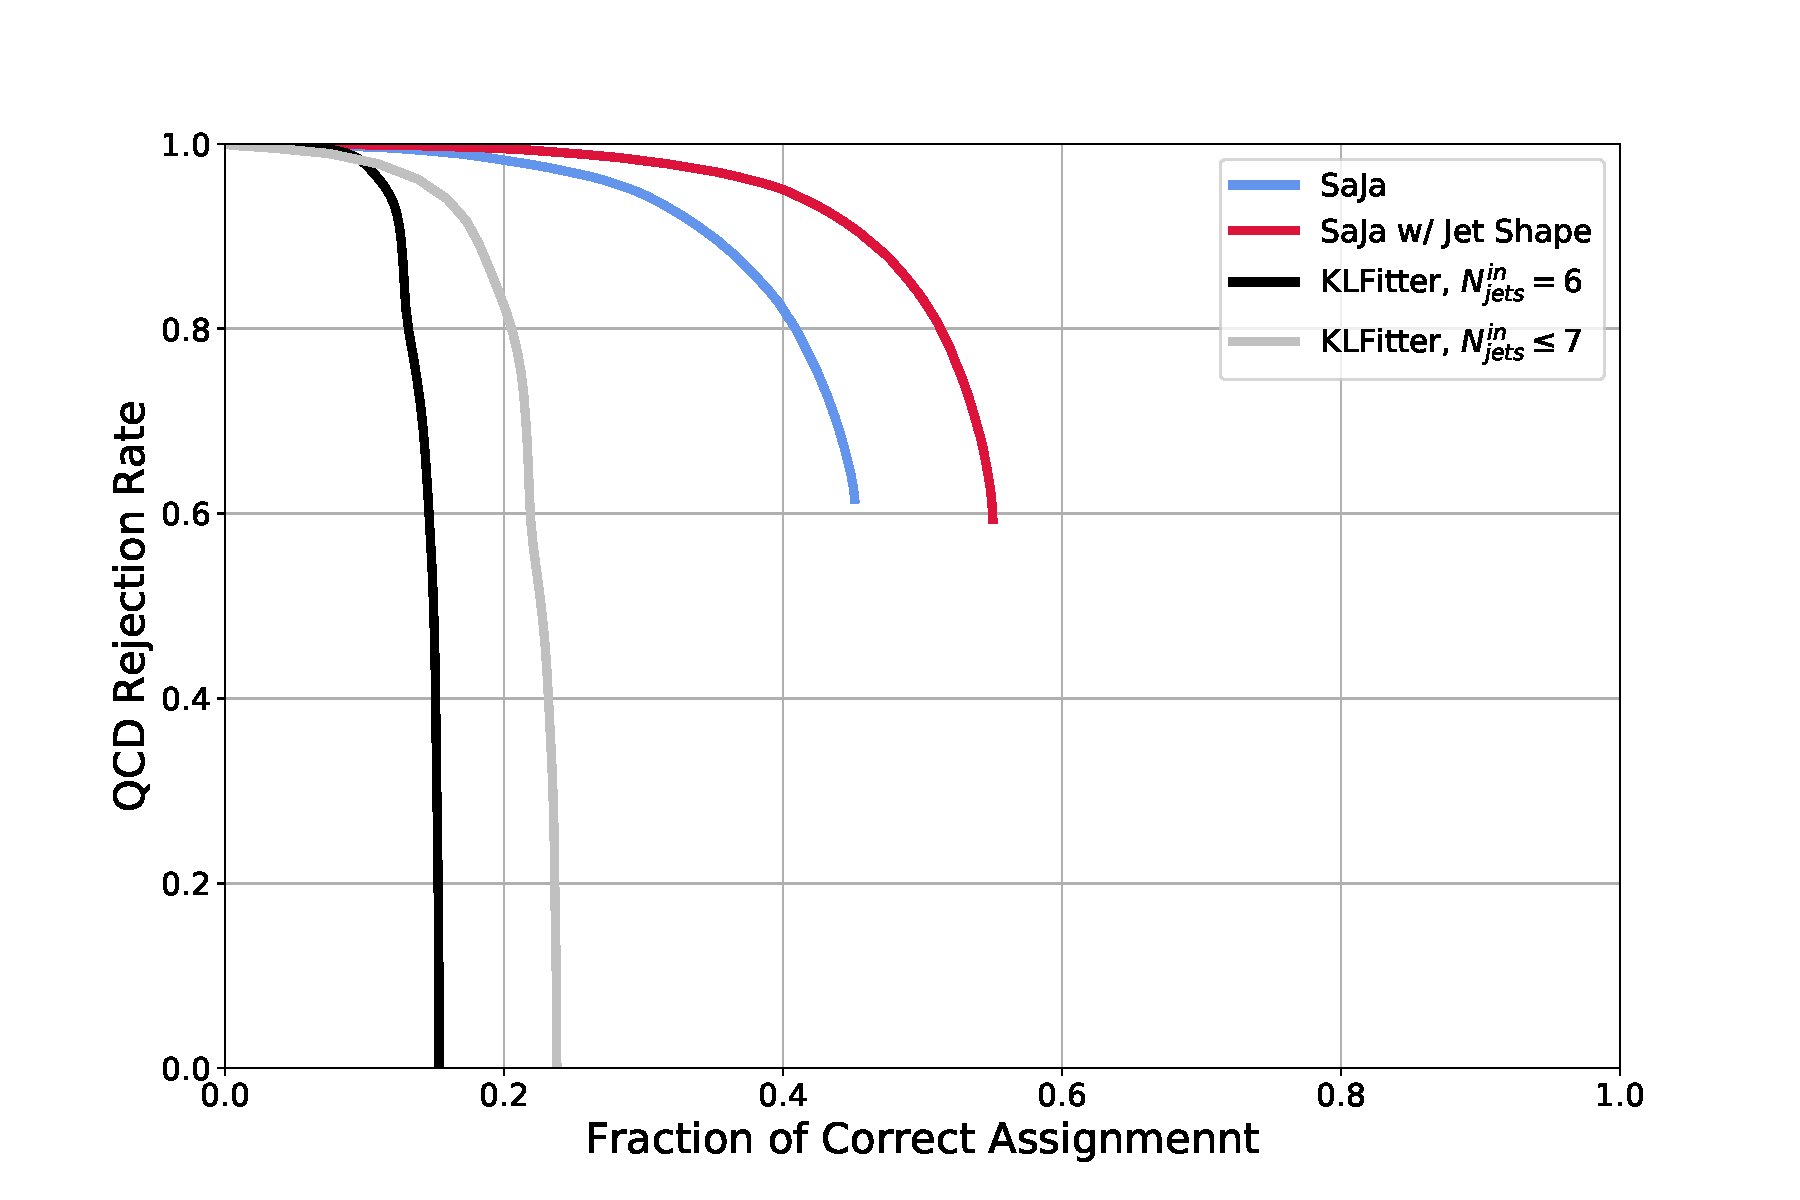
\includegraphics[width=\textwidth]{figures/roc/qcd_rej_vs_mat_tt_acc.pdf}
            \end{figure}
    \end{columns}
\end{frame}


%%%%%%%%%%%%%%%%%%%%%%%%%%%%%%%%%%%%%%%%%%%%%%%%%%%%%%%%%%%%%%%%%%%%%%%%%%%%%%%%



\begin{frame}[fragile]{Model Interpretability}
    \begin{figure}
        \centering
        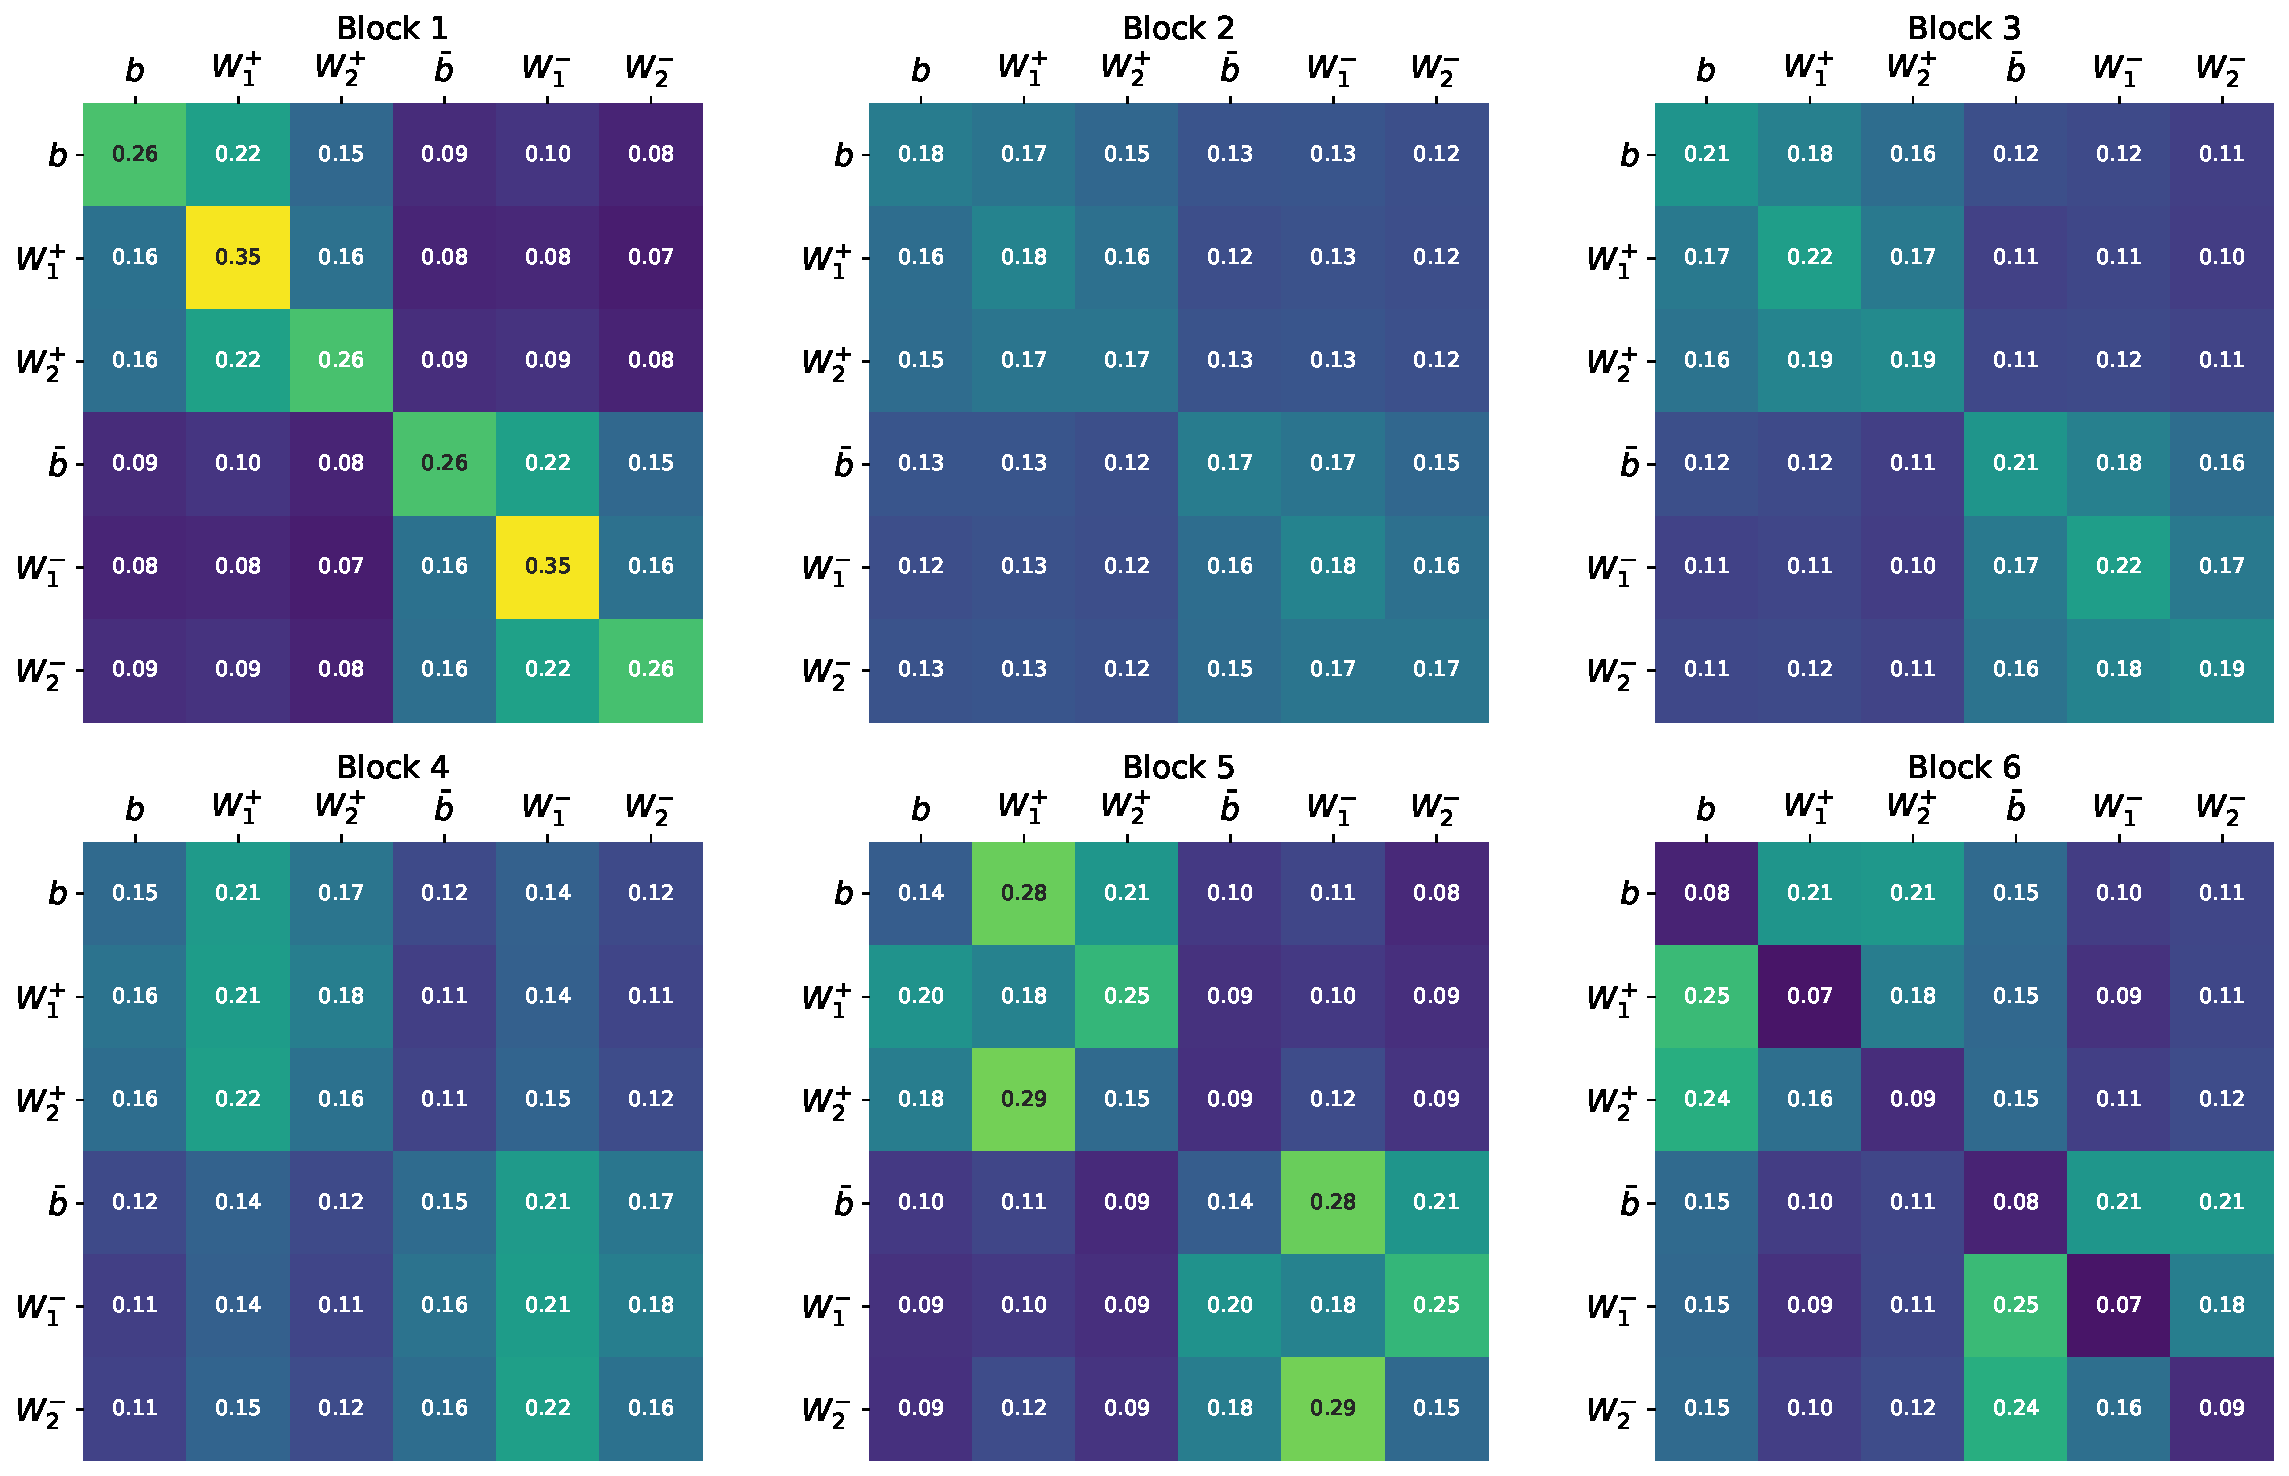
\includegraphics[width=0.75\textwidth]{figures/attention/attention_tt_mg5_pythia8_alljets_dR-0.30_test_delphys_minmax_jet-shape_correct.pdf}
    \end{figure}
    
    {\scriptsize $\bullet$ The average of attention matrices for the correct assignments in the matched $t\bar{t}$ events.}
    \break
    {\scriptsize $\bullet$ Since \saja\, is invariant under the permutation of the jets, it is possible to sort the jets using the jet-parton matching information w.l.o.g., for display purposes.}
    \break
    {\scriptsize $\bullet$ $W_{1}^{+}$ indicates higher $p_{T}$ one of the two quarks, the decay products of $W^{+}$ boson.}
\end{frame}

\begin{frame}[fragile]{Inference Latency}
    \begin{figure}
        \centering
        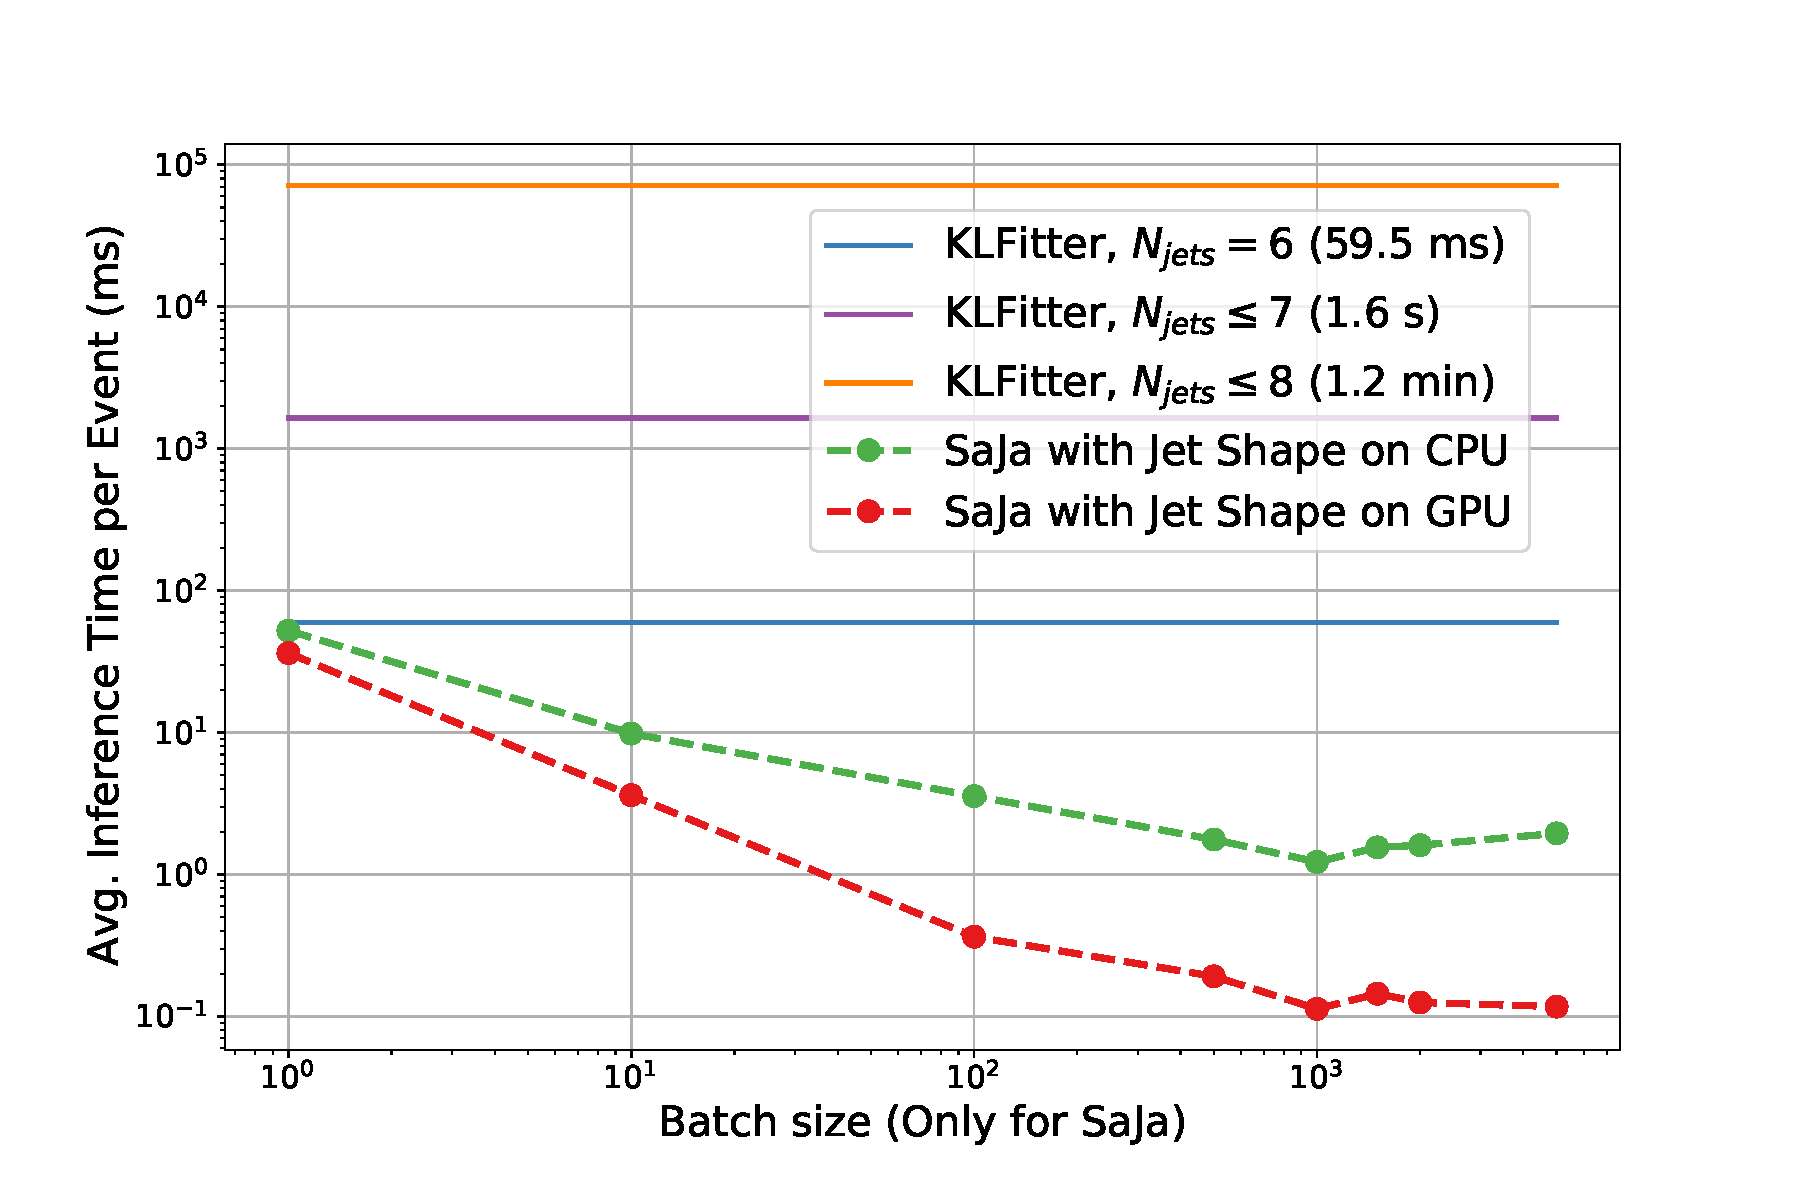
\includegraphics[width=0.6\textwidth]{figures/misc/latency.pdf}
    \end{figure}
    \medskip
    $\bullet$ The graph shows that even for a batch size of one, the zero-permutation \saja\, network is outperforming \textsc{KLFitter}, while a two-order-of-magnitude speed up in inference time is possible by fitting in large batches.
\end{frame}


%%%%%%%%%%%%%%%%%%%%%%%%%%%%%%%%%%%%%%%%%%%%%%%%%%%%%%%%%%%%%%%%%%%%%%%%%%%%%%%%
%
%%%%%%%%%%%%%%%%%%%%%%%%%%%%%%%%%%%%%%%%%%%%%%%%%%%%%%%%%%%%%%%%%%%%%%%%%%%%%%%%

\begin{frame}[fragile]{Summary}
    \begin{itemize}
        \item[$\bullet$] We introduce \textsc{SaJa}\, network for jet-parton assignment without jet permutations.
        \item[$\bullet$] \textsc{SaJa}\, shows better jet-parton assignment and background rejection performance compared to \textsc{KLFitter}.
        \item[$\bullet$] Predictive entropy makes it possible to improve performance without additional training.
        \item[$\bullet$] \textsc{SaJa} is fast even without GPU acceleration.
    \end{itemize}
\end{frame}


\appendix

%\section{Back-up}

%%%%%%%%%%%%%%%%%%%%%%%%%%%%%%%%%%%%%%%%%%%%%%%%%%%%%%%%%%%%%%%%%%%%%%%%%%%%%%%%




\begin{frame}[fragile]{Predictive entropy distribution}
    \begin{figure}
        \centering
        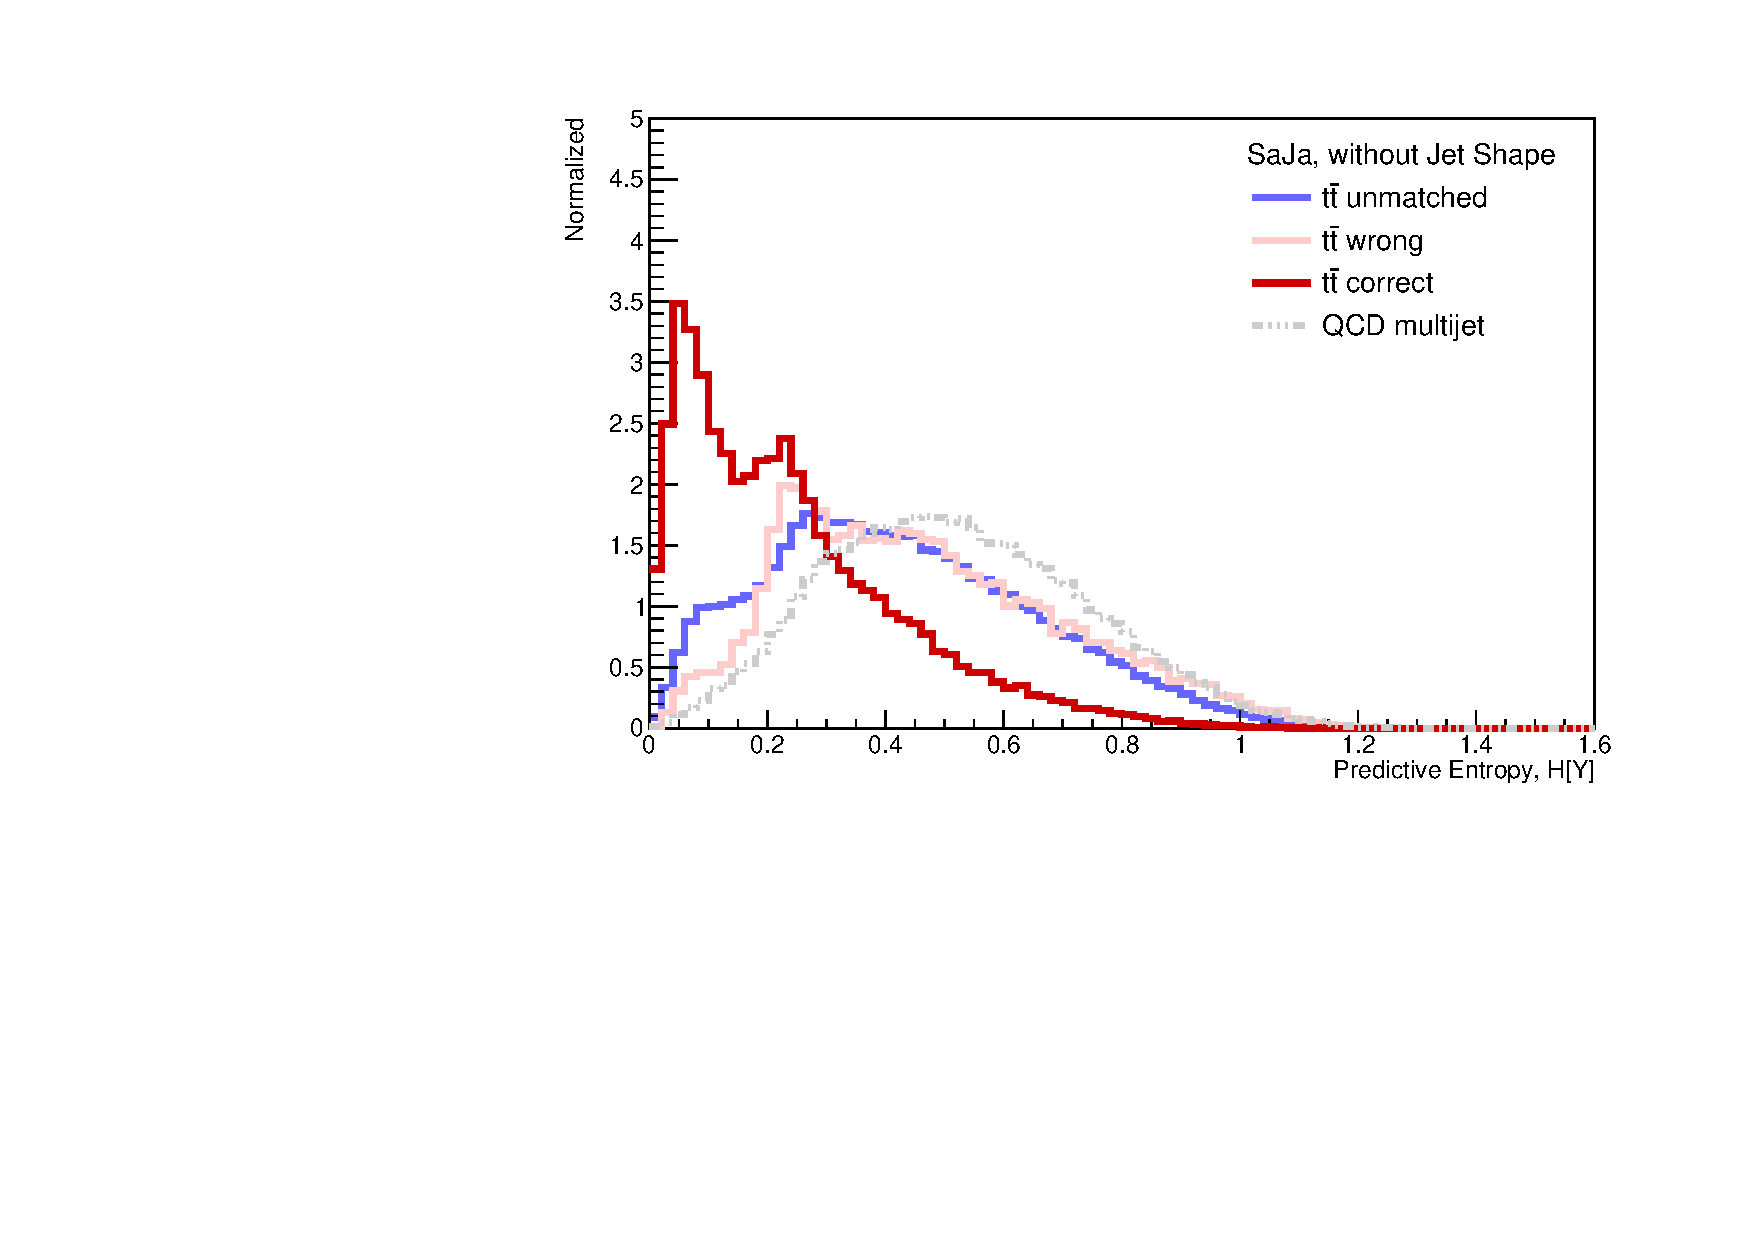
\includegraphics[width=0.45\textwidth]{figures/entropy/entropy_without_jet_shape.pdf}
        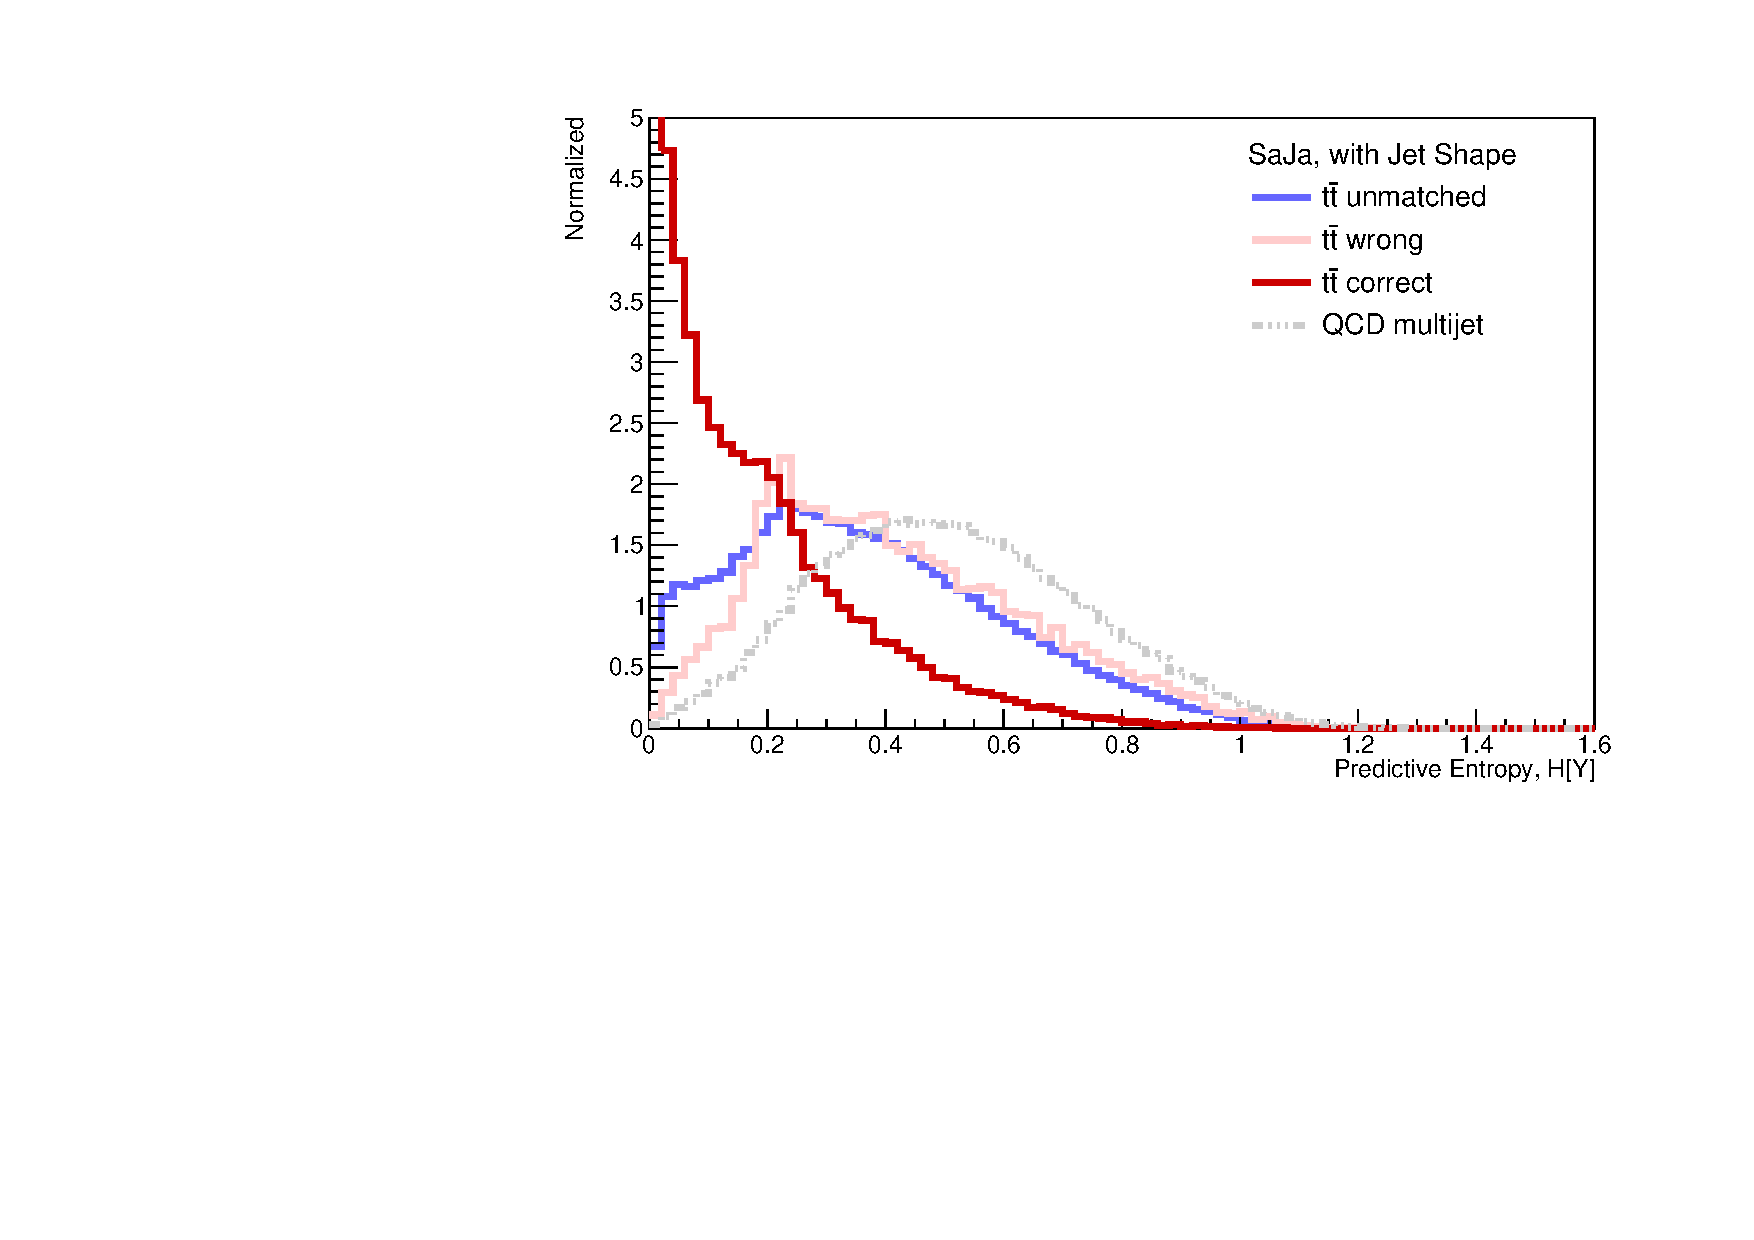
\includegraphics[width=0.45\textwidth]{figures/entropy/entropy_with_jet_shape.pdf}
        %\caption{}
        %\label{fig:my_label}
    \end{figure}
\end{frame}


\begin{frame}[fragile]{Effect of Jet Shape}
    \begin{figure}
        \centering
        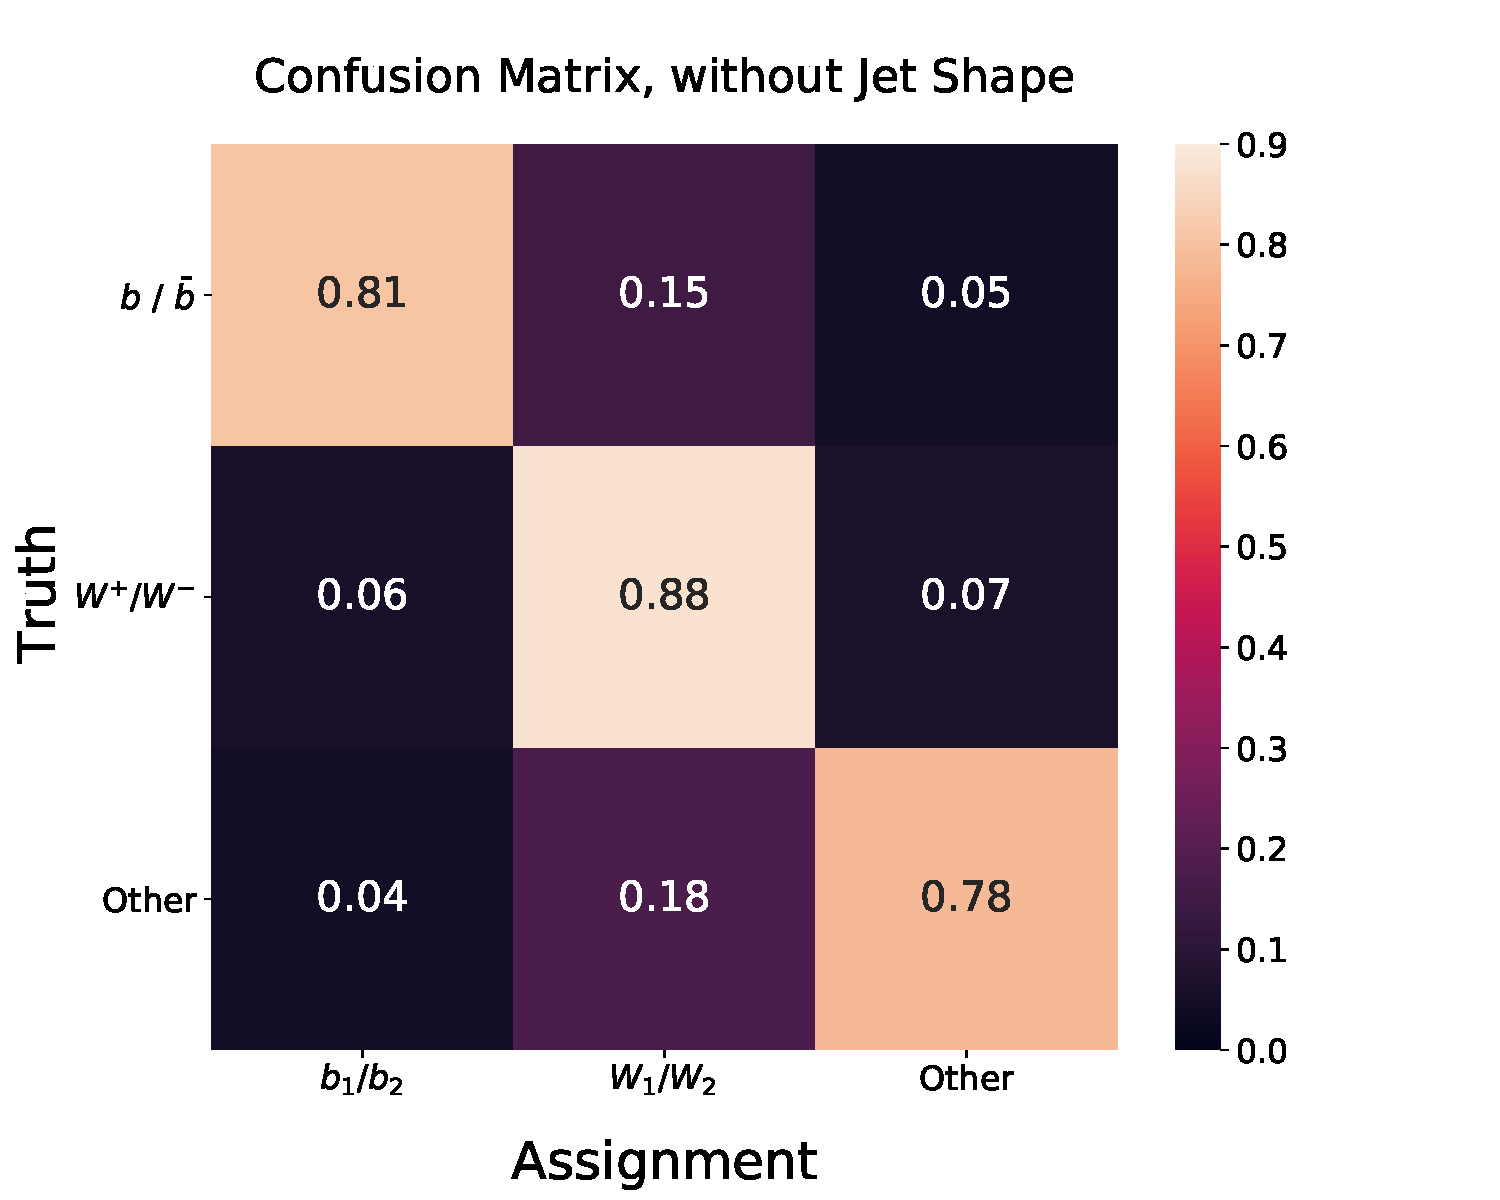
\includegraphics[width=0.45\textwidth]{figures/confusion-matrix/confusion_matrix_without_jet_shape.pdf}
        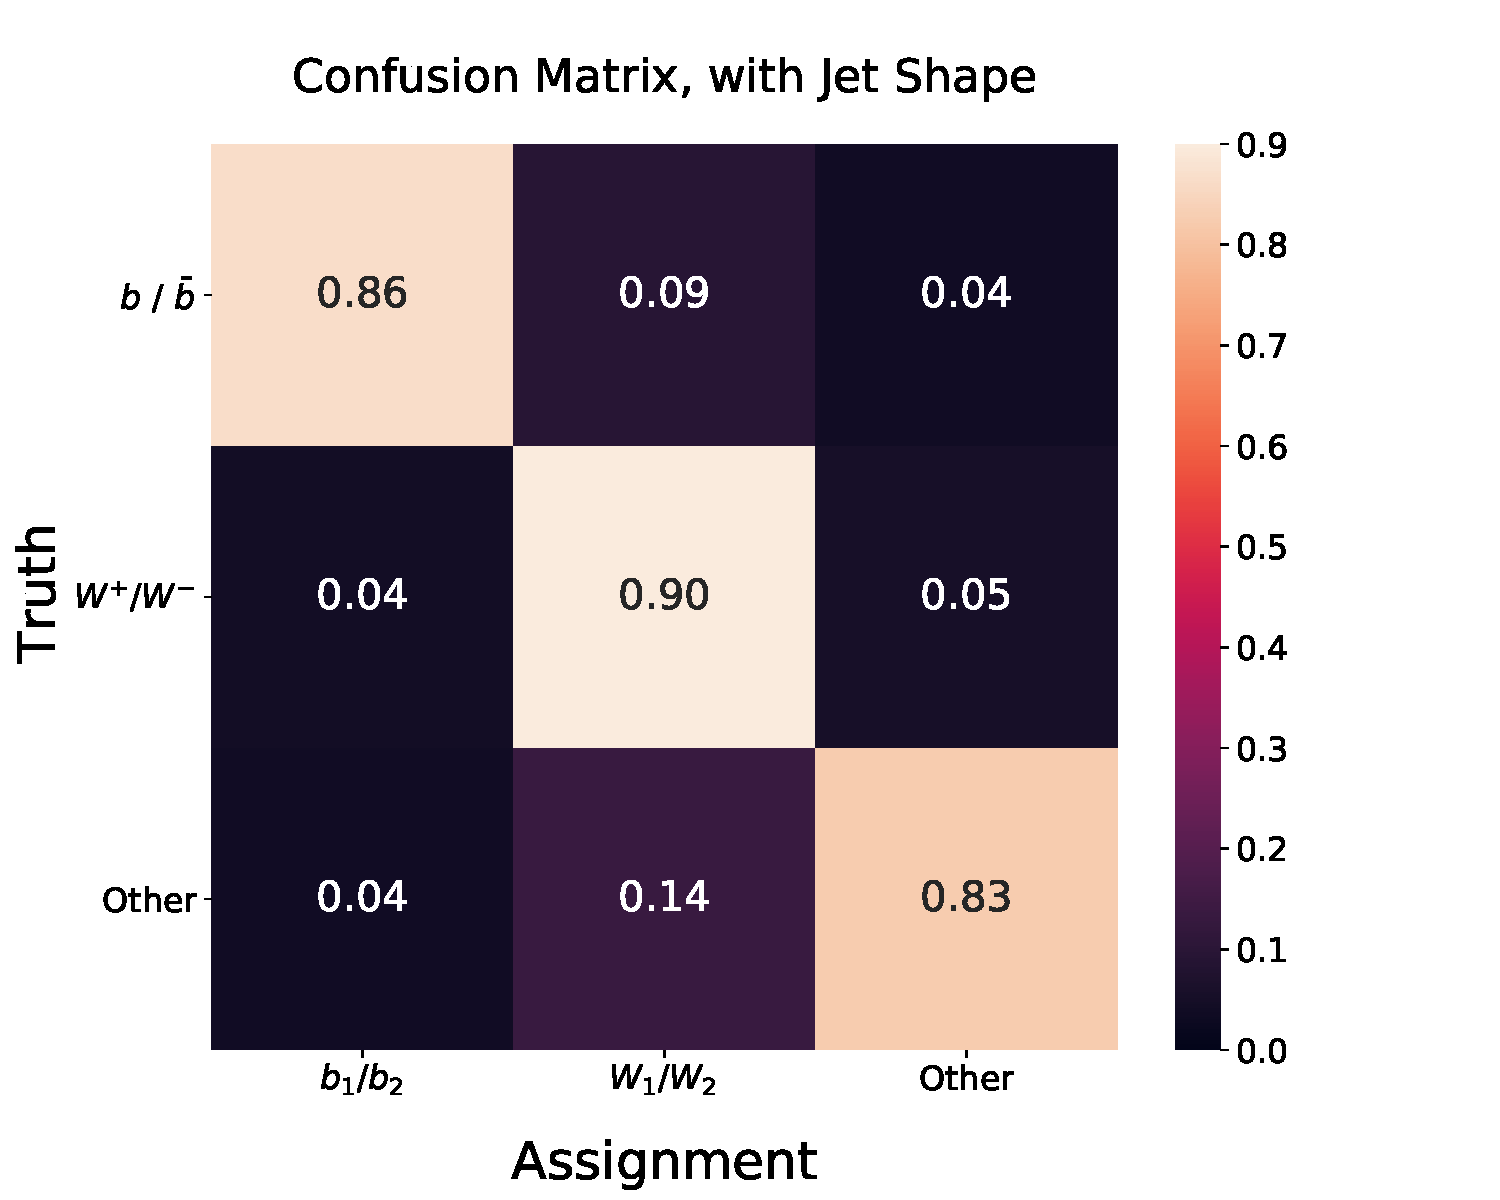
\includegraphics[width=0.45\textwidth]{figures/confusion-matrix/confusion_matrix_with_jet_shape.pdf}
        \caption{Confusion matrices at the jet-level with an without jet shape.}
        %\label{fig:my_label}
    \end{figure}
    Jet shape reduces the case where b-initiated jets and additional jets are assigned to W boson.
\end{frame}

\begin{frame}[fragile]{Fraction of Topologically Valid Assignments}
    \begin{figure}
        \centering
        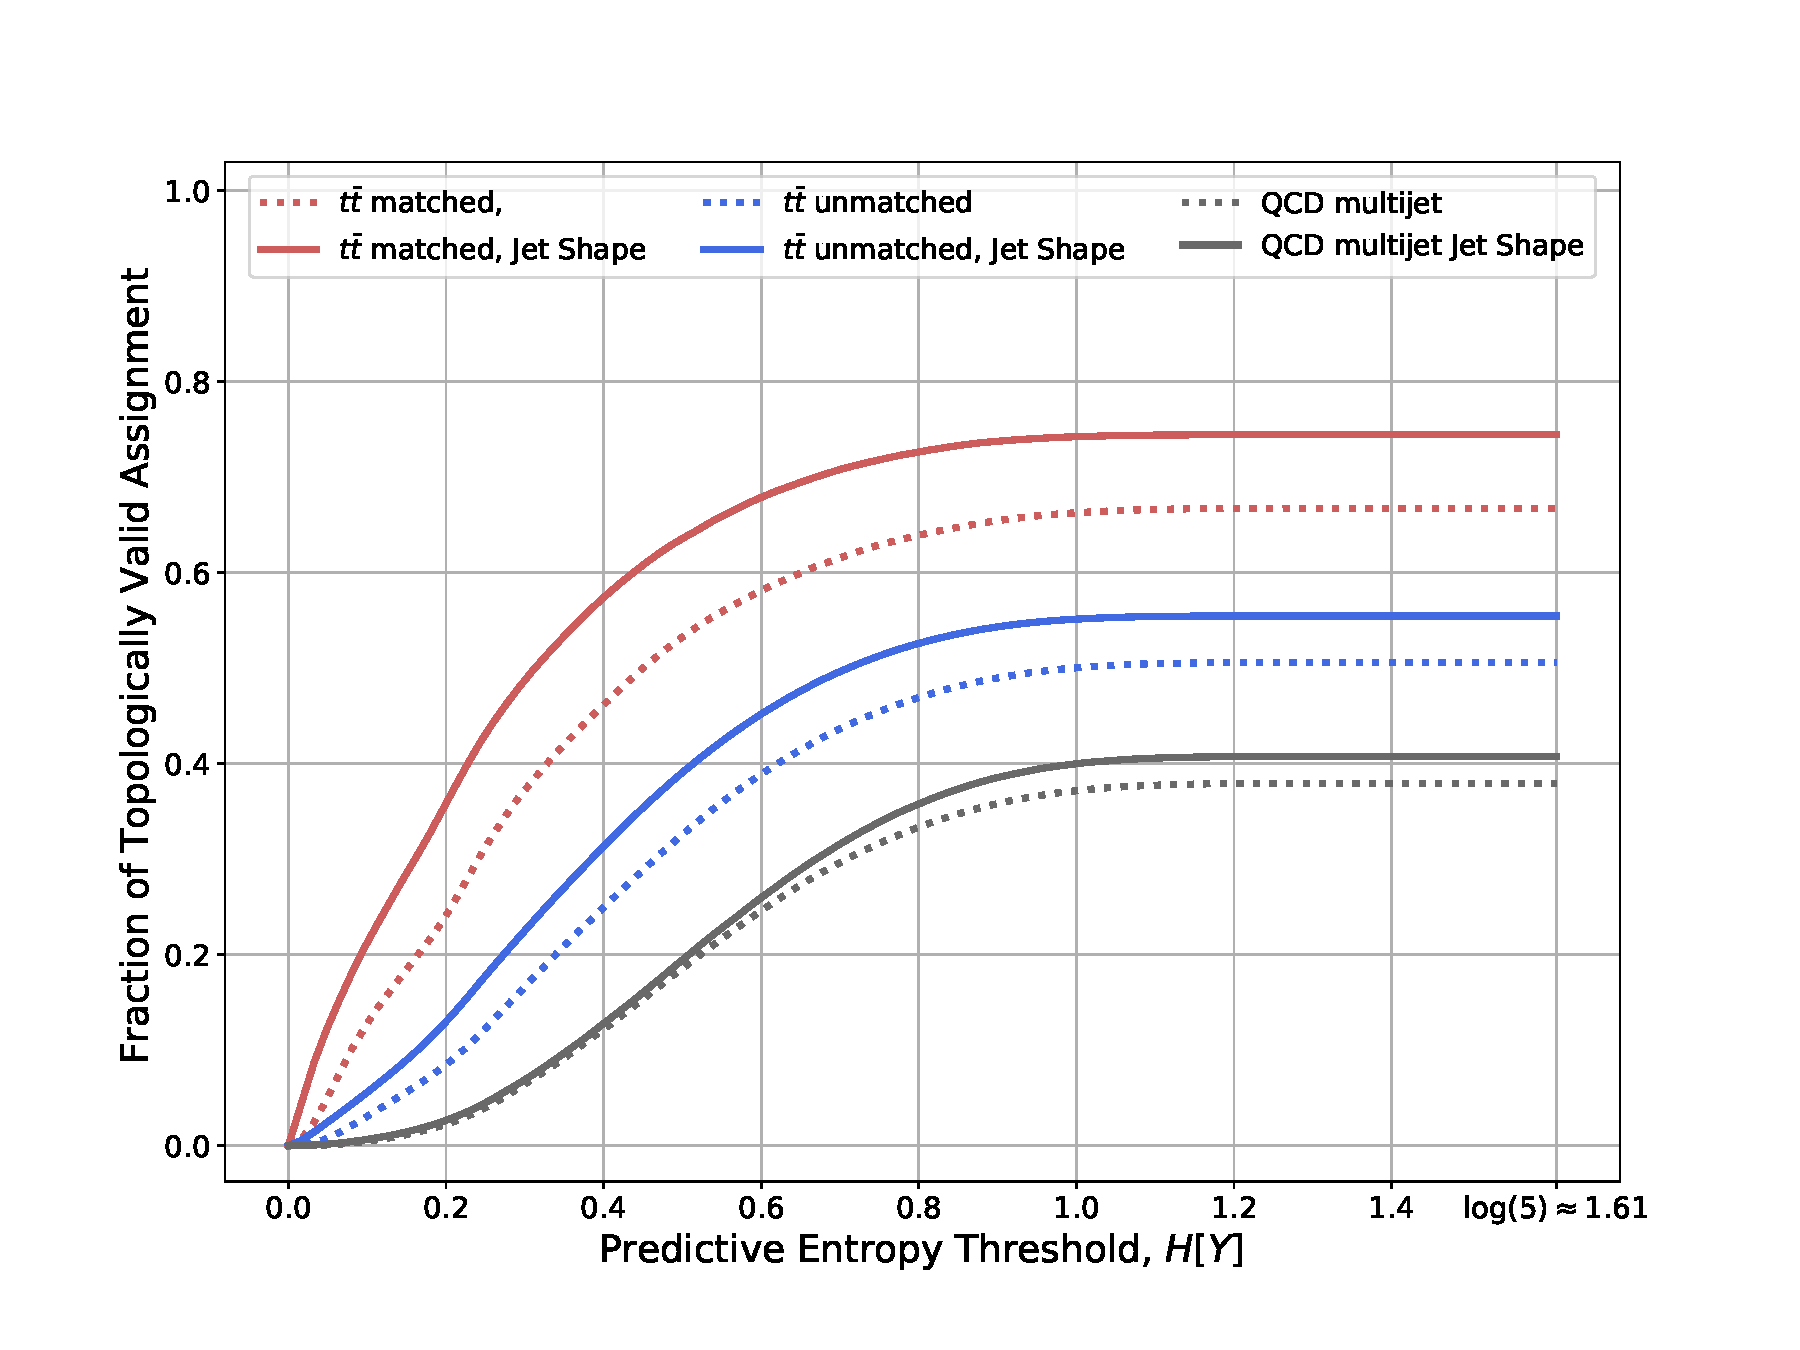
\includegraphics[width=0.8\textwidth]{figures/misc/frac_topo_valid.pdf}
        %\caption{}
        %\label{fig:my_label}
    \end{figure}
\end{frame}



\begin{frame}[fragile]{Training in detail}
    \begin{itemize}
        \item Training, validation, test set: 311k, 80k, 103k events
        \item Adam Optimization algorithm
        \item Learning rate schedule, which reduces the learning rate when the metric on the validation set has stopped improving.
        \item \textsc{PyTorch} v1.3
    \end{itemize}
\end{frame}

\begin{frame}[fragile]{Reconstructed W Boson and Top Quark Mass Distributions}
    \begin{figure}
        \centering
        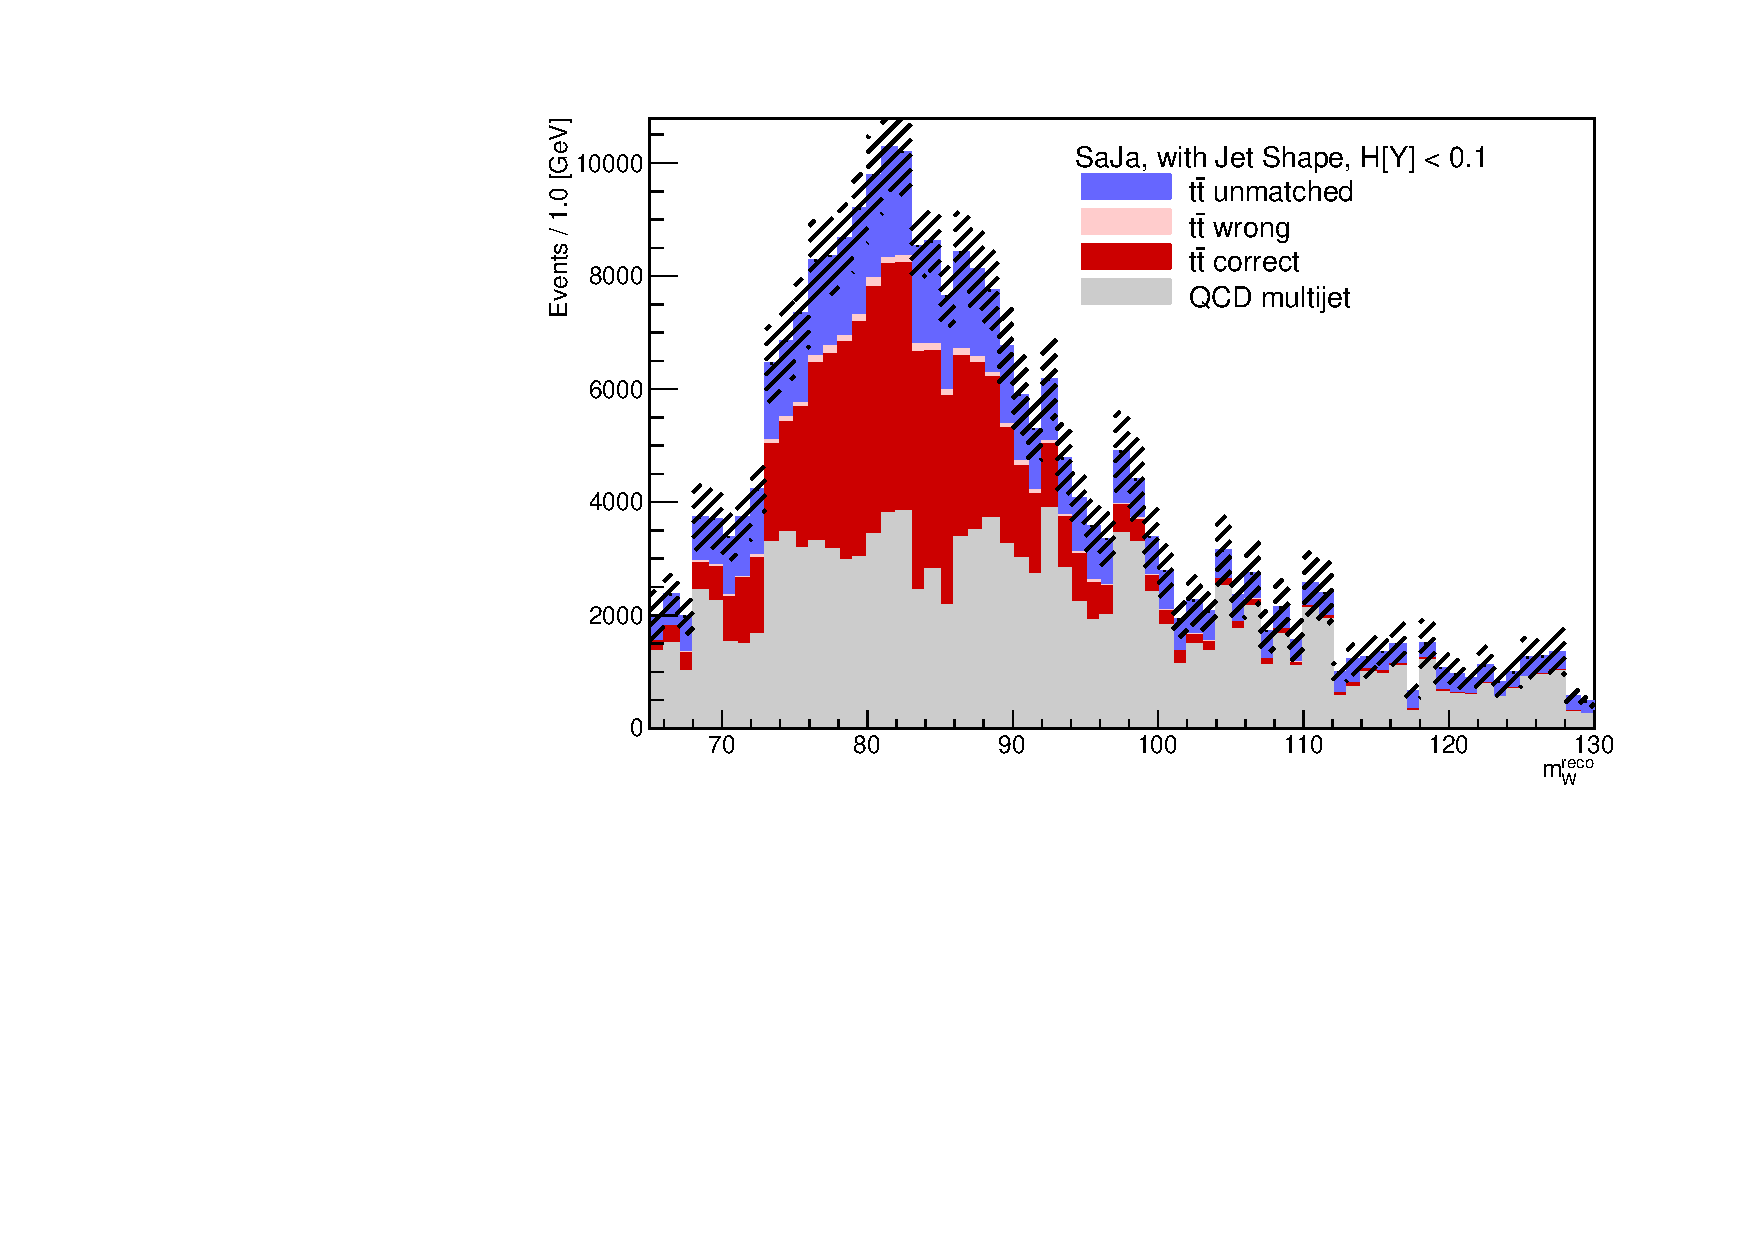
\includegraphics[width=0.48\textwidth]{figures/reco/w_mass_reco_ent-0.10_range-cms.pdf}
        \includegraphics[width=0.48\textwidth]{figures/reco/top_mass_reco_ent-0.10_range-cms.pdf}
    \end{figure}
    (Left) Reconstructed W boson mass distribution and (Right) reconstructed top quark mass distribution.
\end{frame}

\begin{frame}[fragile]{The Effect of Monte Carlo Simulation}
    \begin{figure}
        \centering
        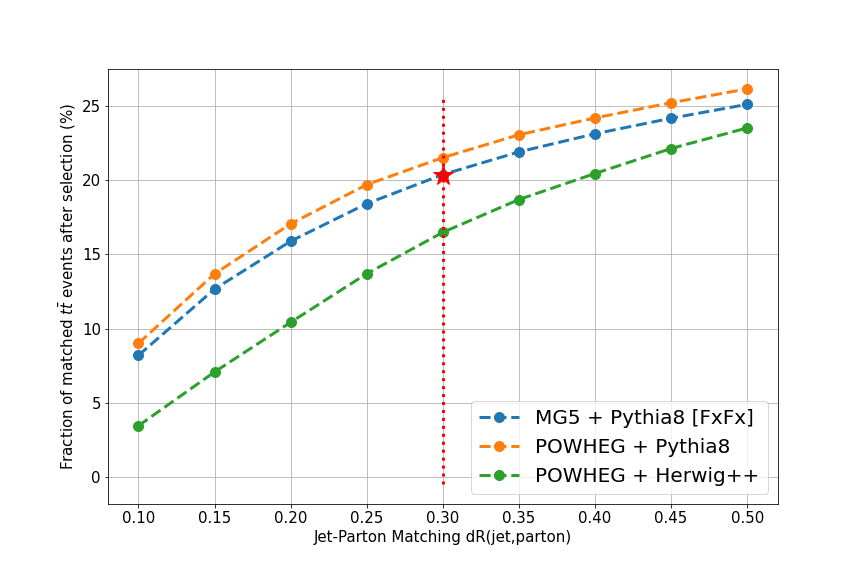
\includegraphics[width=0.48\textwidth]{figures/generator/TotalMinDist-jet-parton-match-by-dR.png}
        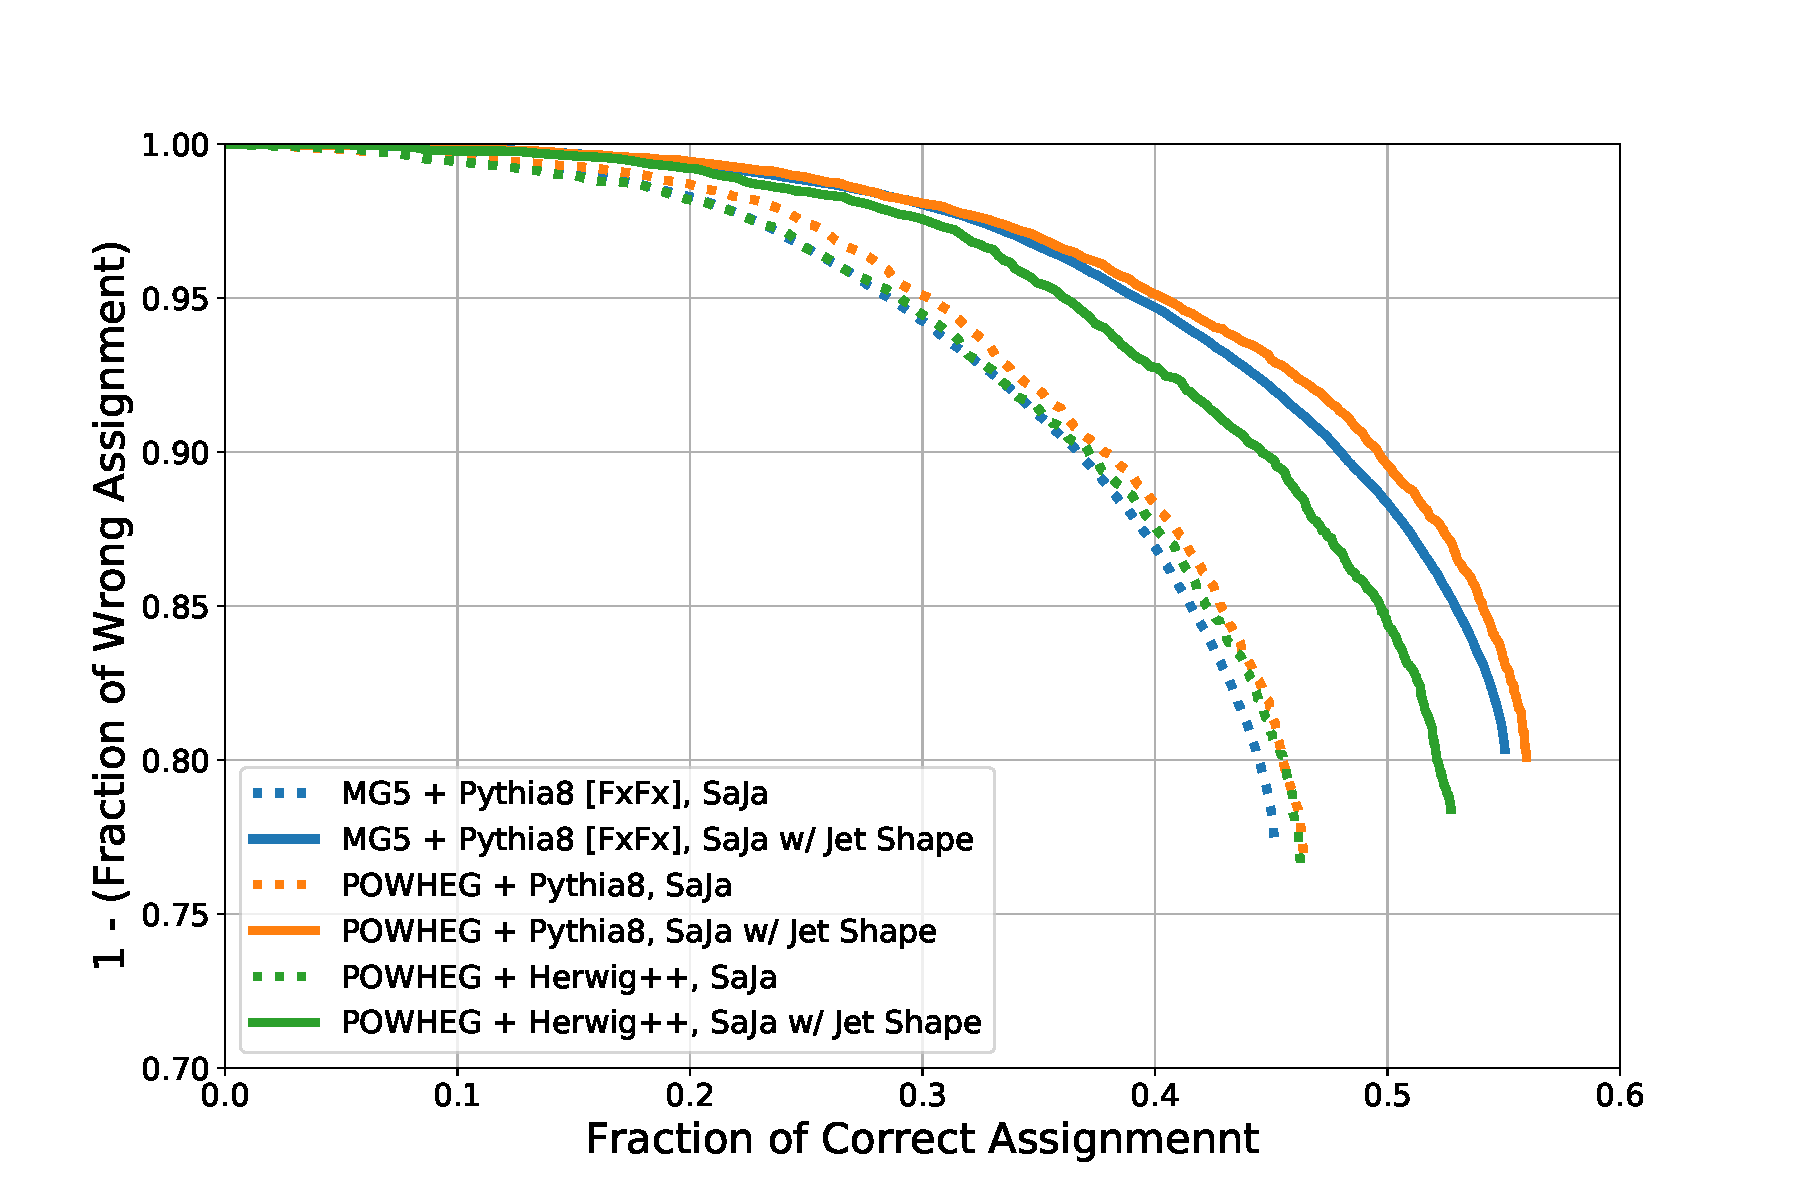
\includegraphics[width=0.48\textwidth]{figures/generator/roc_tt_generator.pdf}
    \end{figure}
\end{frame}


%%%%%%%%%%%%%%%%%%%%%%%%%%%%%%%%%%%%%%%%%%%%%%%%%%%%%%%%%%%%%%%%%%%%%%%%%%%%%%%%

\end{document}
